
%%%%%%%%%%%%%%%%%%%%%%% file typeinst.tex %%%%%%%%%%%%%%%%%%%%%%%%%
%
% This is the LaTeX source for the instructions to authors using
% the LaTeX document class 'llncs.cls' for contributions to
% the Lecture Notes in Computer Sciences series.
% http://www.springer.com/lncs       Springer Heidelberg 2006/05/04
%
% It may be used as a template for your own input - copy it
% to a new file with a new name and use it as the basis
% for your article.
%
% NB: the document class 'llncs' has its own and detailed documentation, see
% ftp://ftp.springer.de/data/pubftp/pub/tex/latex/llncs/latex2e/llncsdoc.pdf
%
%%%%%%%%%%%%%%%%%%%%%%%%%%%%%%%%%%%%%%%%%%%%%%%%%%%%%%%%%%%%%%%%%%%


%\documentclass[runningheads,a4paper]{llncs} % twoside
\documentclass[oneside,a4,12p]{report} %,draft,openright]


\usepackage{amssymb}
\usepackage{amsmath}
\setcounter{tocdepth}{3}
\usepackage{graphicx}
\usepackage{tabularx}
\usepackage{multirow}
\usepackage{multicol}
\usepackage{epsf,graphicx}
\usepackage{epstopdf}
%\usepackage{subfigure}
\usepackage{siunitx}
\usepackage{pbox}
\usepackage{subfig}
\usepackage{color}

\usepackage{url}
\urldef{\mailsa}\path|{alfred.hofmann, ursula.barth, ingrid.haas, frank.holzwarth,|
\urldef{\mailsb}\path|anna.kramer, leonie.kunz, christine.reiss, nicole.sator,|
\urldef{\mailsc}\path|erika.siebert-cole, peter.strasser, lncs}@springer.com|    
\newcommand{\keywords}[1]{\par\addvspace\baselineskip
\noindent\keywordname\enspace\ignorespaces#1}

\begin{document}

%\mainmatter  % start of an individual contribution

% first the title is needed
\title{ Review on Polarization, Imaging Polarimetry and Multispectral Imaging in Biomedical Tissue}

% a short form should be given in case it is too long for the running head
%\titlerunning{Summary on Polarization and Imaging Polarimetry in Biomedical Tissue}

% the name(s) of the author(s) follow(s) next
%
% NB: Chinese authors should write their first names(s) in front of
% their surnames. This ensures that the names appear correctly in
% the running heads and the author index.
%
\author{Mojdeh Rastgoo}
%\thanks{Please note that the LNCS Editorial assumes that all authors have used
%the western naming convention, with given names preceding surnames. This determines
%the structure of the names in the running heads and the author index.}%
%\and Ursula Barth\and Ingrid Haas\and Frank Holzwarth\and\\
%Anna Kramer\and Leonie Kunz\and Christine Rei\ss\and\\
%Nicole Sator\and Erika Siebert-Cole\and Peter Stra\ss er}
%%
%\authorrunning{Summary on Polarization and Imaging Polarimetry in Biomedical Tissue}
% (feature abused for this document to repeat the title also on left hand pages)

% the affiliations are given next; don't give your e-mail address
% unless you accept that it will be published
%\institute{Springer-Verlag, Computer Science Editorial,\\
%Tiergartenstr. 17, 69121 Heidelberg, Germany\\
%\mailsa\\
%\mailsb\\
%\mailsc\\
%\url{http://www.springer.com/lncs}}

%
% NB: a more complex sample for affiliations and the mapping to the
% corresponding authors can be found in the file "llncs.dem"
% (search for the string "\mainmatter" where a contribution starts).
% "llncs.dem" accompanies the document class "llncs.cls".
%
%
%\toctitle{Lecture Notes in Computer Science}
%\tocauthor{Authors' Instructions}
\maketitle
\bibliographystyle{splncs03}

%%\begin{abstract}
%%Polarization is one of the fundamental properties of light and could be used as the basic concept of imaging. Imaging polarimetry which is based on the polarization concepts could be used to highlight the characteristics of the incident light or the material itself. This report represents the classical theory of polarization, imaging polarimetry and the application of imaging polarimetry with special interest in biological tissues.
%%\end{abstract}



%%%%%%%%%%%%%%%%%%%%%%%%%%%%%%%%%%%%%%%%%%%%%%%%%%%%%%%%%%%%%%%%%%%%%%%%%%%%%%
%%% CHAPTER 1
%%%%%%%%%%%%%%%%%%%%%%%%%%%%%%%%%%%%%%%%%%%%%%%%%%%%%%%%%%%%%%%%%%%%%%%%%%%%%

%\chapter{Skin Data Analysis}
%In this chapter first the anatomy of human skin, then the cutaneous melanoma and its different types as well as its clinical diagnosis are discussed. Later common imaging techniques for diagnosis of melanoma are discussed. Finally at the end skin optical properties and different methods for modeling light propagation through skin are reviewed. 
%
% 	\section{Human Skin}
%
%	The description and understanding of human skin physiology and anatomy is required in order to model the light propagation through the skin. Skin is the largest organ of human body and consists of three main layers, epidermis, dermis and subcutaneous fat  \cite{anderson1981optics} (see Fig.\ref{fig:SkinAnatomy}).\\
%		\begin{figure}
%		\centering
%		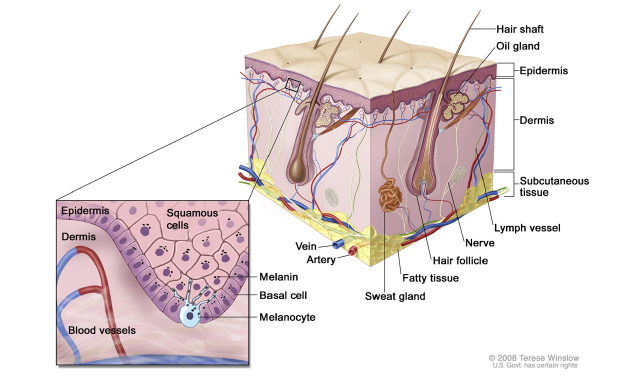
\includegraphics[width = 0.6\textwidth]{figures/SkinAnatomy.png}	
%	\caption{Anatomy of the skin, showing the three structure layer of epidermis, dermis and subcutaneous tissue \cite{korotkov2012computerized}}
%		\label{fig:SkinAnatomy}
%		\end{figure}	 
%
%	\textbf{Epidermis} contains the outer layer and surface of the skin. This layer is d into five sublayers, such as stratum corneum, stratum basale, stratum spinosum, stratum granulosum and stratum lucidum. Four different cells are found in these layers including: 
%	\begin{itemize}
%	\item \textit{Keratinocytes}. Majority of the cells in epidermis belong to this group which are the main force for continuous renewal of the skin. These cells contain two main features of division and differentiation. These properties enable them to renew the outer layer of the epidermis within each thirty days. 	
%%	These cells poses the properties of division and differentiation which enable them to take the thirty days journey for renewal of the outer layer of the epidermis.
%During this journey, the daughter keratinocytes, which is produced by division of the basal cells (keratinocytes in basal layer are called basal cells) will move to the next layer while its going through differentiation process. Differentiation refers to morphology and biochemistry transformation of the cells. As the result of this process, the keratinocytes cells are transformed to flattened cells without nuclie filled with keratine. These cells form the outer most layer of the epidermis which is called corneocytes. At the end of differentiation program the corneocytes lose their cohension and separate from the surface in the desquamation process. \\
%
%
%%This process is referred to transformation of the cell in terms of its morphology and biochemistry. 
% 
%%During this journey, the daughter keratinocytes produced by division in the basal layer (here they are called as basal cells) will move to the next layer while transforming its morphology and biochemistry (differentiation process). As a result of this movement and transformation, the flattened cells without nuclei filled with keratine come to form the outer most layer of the epidermis and called corneocytes. Finally in the end of differentiation program the corneocytes lose their cohension and separate from the surface in the desquamation process. \\
%
%
%\item \textit{Melanocytes}. Dendritic cells found in the basal layer of epidermis. These cells are responsible for distributing packages of melanin pigment to surrounding keratinocytes, which leads to individual skin and hair colors. Melanin is the major chromophore of the epidermis which occupies the top 50-100 \micro\meter , with the exception to superior layers of epidermis. Melanin is produced by melanosomes when exposed with UV light and is divided into two types of eumelanin and pheomelanin. Eumelanin has black/brown colour while pheomelanin has red/yellow colour. Concentration of this components are different between individuals, leading to different colour skins.\\
%	
%\item \textit{Langerhans}. These cells are dendritic like melanocytes. They are responsible for detection of foreign bodies (antigens) which have invaded into epidermis and transporting them to the local lymph nodes.\\
%
%
%\item \textit{Markel}. These cells act as mechanosensory receptors in response to touch. 
%
%\end{itemize}
%
%	In most of light propagation models through skin, the sublayers of epidermis are considered as one layer. Epidermis thickness could vary depending on different body parts, however in average it is mentioned to be 0.1 mm. The most external sublayer of epidermis is stratum corneum which is composed of dry dead cells without organelles and is filled with keratin fibres. The light is mainly absorbed in this layer, due to epidermis major component melanin.\\	
%%	The epidermis main effect on the light is absorption due to its major component, melanin. \\
%
%	\textbf{Dermis} is the middle layer between epidermis and hypodermic layer. This layer is thicker than epidermis, with an average thickness of 0.6 to 3 mm \cite{anderson1981optics}. The thermoregulation, mechanical resistance and nourishing of the epidermis are the main function of this layer. Dermis is composed of elastic collagen fibres, blood vessels, nerves, lymph vessels, hair follicles and sweat glands but the principal molecules with interesting optical properties are the haemoglobin, carotene and bilirubin. 
%Haemoglobin is a chromophore of red colour found in the microvascular network of the dermis, typically 100-500 \micro\meter  below the skin surface. This chromophore caries oxygen through vessels and capillaries and accordingly is called oxy-haemoglobin while it contains oxygen and deoxy-haemoglobin otherwise. 
%
%Dermis is divided into two sublayers, papillary dermis with principal function of thermoregulation and reticular dermis which gives the skin its strength and elasticity. \\
%
%\textbf{Subcutaneous fat} or hypodermic is the deepest layer of the skin, with the average thickness from 4 to 9 mm. This layer is composed of connective tissues, fat cells and blood vessels. 
%
%
%	\section{Melignant Melanoma}
%
%	Cancer can develop from almost any cell in the body, however certain cells are more cancer prone compare to others and the skin is not an exception. Most skin cancers develop from non-pigmented cells and not from pigmented melanocytes \cite{Kaufman2005}. The three most common malignant skin cancers are called basal cell carcinoma, squamous cell carcinoma and melanoma which develop from basal, squamous keratinocytes and melanocytes accordingly. 
%Although Melanoma is less common in comparison to basal cell carcinoma and squamous cell carcinoma, however it is the most dangerous and deadly type of skin cancer. Melanoma causes the majority of deaths related to skin cancer \cite{Kaufman2005,Markovic2007}. This cancer is found incurable in its advanced stages and in foremost stages the treatment is limited to surgery, immunotherapy, chemotherapy and/or radiation therapy. %(with evidence of metastasis)
%Although melanoma can be deadly in its late stages, it could be treated easily in its early stage. Due to this statistics, majority of research are carrying on in this field, with the aim of early detection and diagnosing of the cancer. In the following first a classification of melanoma and then the clinical diagnosis are discussed. % in order to improve early detection and diagnosis of the cancer in the pigmented lesion. 
%
%	\subsection{Melanoma Classification}
%	Melanoma is usually a cancer of skin, however the general term of melanoma includes three different cancer, such as, cutaneous melanoma, mucosal melanoma and ocular melanoma. The cutaneous melanoma is the most common type, and defines one category of skin cancers. The other category of skin cancer is named Non-Melanoma and includes, basal cell carcinoma and squamous cell carcinoma. As opposed to melanoma this category normally do not spread to other body parts. \\
%	
%	The cutaneous melanoma consists of four basic types. The first three type begin \textit{in situ}, meaning that they spread in the top layers of the skin and in last stages they become invasive, while the fourth one is invasive from the start. Invasive melanoma could be more dangerous since they are in deeper layer of the skin and they can spread faster to other body parts \cite{malonacenter}. The four types of cutaneous melanoma are listed in the following \cite{malonacenter,MelanomaResearchFoundation} 
%	
%	\begin{itemize}
%	\item Superficial Spreading Melanoma	\\ 
%	This is the most common type and is the leading cause of cancer death in young adults. Approximately 70\% of all melanoma diagnosis is counted as superficial spreading melanoma. This type grows along the top layer of the skin and often occurs in a previously benign mole. The location of this melanoma can be anywhere in the body, however it is usually located on the trunk and back in male patients and on the legs and back in females patients.   
%	
%	\item Acral Lentiginous Melanoma\\
%	This group accounts for less than 5\% of all melanomas diagnosis and is the most common type in dark skin individuals. This disease usually is located on the palms, soles of the feet and under the finger nails and often look like a bruise or injuries on the body. Due to this matter this melanoma may be discovered later than other forms.  
%	
%	
%	\item Lentigo Maligna Melanoma\\
%	Five to ten percent of the melanoma diagnosis belongs to this group. Letigo maligna melanoma arises from a pre existing lentigo rather than a mole and mostly occurs on the face of middle-aged to elderly individuals as a result of sun damage. 
%If this cancer stay undiagnosed being mistaken with sun spot it can spread to the deep layers of skin and danger the patients life. The cancer lesions of this type, usually have a very irregular border and vary in shades of brown or black however like other types of melanoma, they can be blue, red, gray or white. 
%
%	\item Nodular Melanoma\\
%Almost 15\% to 30\% of all melanoma diagnosis counts for nodular melanoma. This is the most aggressive type due to the fact that it spreads more rapidly in depth and it is difficult to visualize the progression of the cancer.
%Nodular melanoma is more common in males compared to females. The lesion is usually darkly pigmented (blue-black) and often is found in pink or red. 
%	\end{itemize}
%	
%	
%	\subsection{Clinical Diagnosis}
%	%% ABCD, ABCDE, 7 check point list , Biopsy, Melanoma stages, staging factors
%Due to visible nature of melanoma disease, visual inspection of the lesions is the first step of diagnosis. The visual inspection is based on certain criteria with the aim to differentiate between benign and suspicious lesions. In 1985 Friderman et al. \cite{Friedman1985} introduced ``ABCD'' criteria for identifying melanoma. This method introduced simple criteria for appraise of one lesion such as Asymmetry, Border irregularity, Color variegation and Diameter greater than 6 mm.  Due to its simple definition of the criteria, this method have been used widely in clinical practice. However later in 2004, Abbasi et al. \cite{Abbasi2004} proposed expanding the ``ABCD'' criteria to ``ABCDE'', while E stands for evolving the lesion over time with respect to size, shape, shades of color, surface features or symptoms. \\
%
% Clasgow 7-point checklist \cite{Mackie1991} is another melanoma identification method in clinical diagnosis. This method considers three major criteria such as changes in size, shape and colors and four minor criteria, including diameter greater than 7 mm, inflammation, crusting or bleeding and sensory change. Opposed to ABCDE and ABCD, Glosgow 7 point checklist is not widely adopted and the used of the former method is more evident in the state of the art. 
% 
%%%Beside what is mentioned here, it is often to see the same technical terms (ABCD and 7-point checklist) in the literature, while they stand for different image modalities \cite{korotkov2012computerized}. For instance in the ABCD rule of dermoscopy, B stands for Border sharpness and D for Differential structure.  
%
%All the mentioned methods are used by the dermatologists and non dermatologists to identify suspicious lesions and differentiate the benign melanocytic tumors from melanoma. The suspicious lesions are removed by biopsy and special measurements are conducted for evaluating the risk factor of the lesion.
%
%
% Based on American Joint Commission on Cancer (AJCC) (7th edition on melanoma staging and classification) \cite{balch2009final}, 10 different stages of melanoma are recognized in clinical and pathological used. This information is shown in Table \ref{T:Melanoma Sataging}. According to \cite{balch2009final}, there are several factors for determining the stage of melanoma and its indication, such as: 
%	\begin{itemize}
%	\item T- Tumor thickness. This factor varies from 1 - 4 and depending on the presence or absence of ulceration have different notation (b-a, respectively).
%	\item N- Nodes (Lymph). This factor has 4 forms (0-3) and indicates if the melanoma has spread to lymph nodes.
%	\item Metastasized. This factor points out if the cancer spread to other organs.
%	\item Mitotic Rate, This parameter corresponds to the ratio of cell numbers in mitosis to total amount of cells and it is expressed as the number of mitoses/mm2.  
%	\end{itemize}
%
%
%	\begin{table}
%	\small
%	\caption{Melanoma Stages\cite{balch2009final}}
%	\begin{center}
%		\begin{tabular}{|c|p{8cm}|}
%		\hline
%		 Stage & Description \\ \hline
%		 & \\
%		 0 &  The tumor is bound to the epidermis and has not entered the dermis\\
%		 & \\
%		 IA & The tumor is less than 1 mm thick without ulceration (\textit{T1a}) and it has not spread to any other lymph nodes or organs (\textit{N0}, \textit{M0})\\
%		  & \\
%	     IB & The tumor is either less than 1 mm with the presence of ulceration (\textit{T1b}) or 1-2 mm and without ulceration (\textit{T2a}) and it is not spread to any other lymph nodes or organs (\textit{N0}, \textit{M0})\\
%		 & \\
%         IIA & The tumor is either between 1-2 mm and ulcerated (\textit{T2b}) or 2-4 mm thick and not ulcerated (\textit{T3a}. The tumor is not extended to other lymph nodes or organs (\textit{N0}, \textit{M0})\\
%		 & \\
%		 IIB & The tumor thickness is either 2-4 mm while ulcerated (\textit{T3b}) or more than 4 mm and not ulcerated (\textit{T4a}). The tumor has not spread to any lymph nodes or organs (\textit{N0}, \textit{M0})\\
%		 IIC & The tumor is more than 4 mm thick and ulcerated (\textit{T4b}). The tumor has not extended yet to other parts of the body (\textit{N0}, \textit{M0})\\
%		 & \\
%         \pbox{2cm}{IIIA\\IIIB\\IIIC} & In this stage the tumor can be any thickness with presence or absence of ulceration (\textit{T $>$ T0}). The tumor has not spread to any other organs (\textit{M0}), however it is extended to the surrounded lymph nodes (\textit{N $>$ N0}).\\
%         IV &  The cancel cells are extended to the other nodes and body organs. \\
% 
%         \hline
%				  
%		\end{tabular}
%    \end{center}
%	\label{T:Melanoma Sataging}	
%	\end{table}	 
%  
%The mentioned factors are used to classify and stage melanoma, however two common indicators are mostly used to evaluate the progression of melanoma \cite{balch2009final}, including: 
%
%	\begin{itemize}
%	\item Clark's level\\
%	The clark's level indicate the depth that the tumor is penetrated into the skin. Although it was shown that this diagnosis was not a great indicator, it is still used along the Breslow thickness. 
%		\begin{itemize}
%		\item Clark's level I - Bound to the epidermis (\textit{in situ} melanoma)
%		\item Clark's level II - Confined to the upper part of papillary dermis 
%		\item Clark's level III - Filling to the lower part of papillary dermis
%		\item Clark's level IV - Invading to the reticular dermis
%		\item Clark's level V - Expanding to the subcutaneous tissue
%		\end{itemize}	
%	
%	\item Breslow thickness\\
%The Breslow thickness indicates the vertical depth of the tumor in millimetres. This continuous factor is more accurate compare to Clark's level and is measured using an instrument called ocular micrometer \cite{balch2009final}. 
%The research has shown there is a common relation between the Breslow thickness and the survival rate. 
%		\begin{itemize}
%		\item Breslow thickness $<$ 1 mm, 5- year survival is 95-100 \%
%		\item 1 mm $<$ Breslow thickness $<$ 2 mm, 5- year survival is 80-96 \% 
%		\item 2.1 mm $<$ Breslow thickness $<$ 4 mm, 5- year survival is 60-75 \%
%		\item Breslow thickness $>$ 4 mm, 5- year survival is  37-50 \%
%		\end{itemize}
%	\end{itemize}
%
%	\section{Imaging Techniques}
%	%for the diseases altering its appearance.
%	Skin is the largest organ of the body and can be examined directly by specialists. Due to this nature, visual inspection is the first procedure performed by dermatologists. In order to achieve spatially, uniform information for diagnostic purposes, different non-invasive imaging systems have been used in this field. These techniques allow the visualization of different skin structures however depending on their portability and ease of access by dermatologists, some have been used in daily basis, while the others are mostly used for research purposes. 
%	The imaging systems based on ultraviolet (UV), visible (VIS), and near-infrared (NIR) spectrum, such as digital imaging, dermoscopy, multispectral, spectrophotometer and hyperspectral systems belong to the former group, while other imaging techniques including, optical coherence tomography (OCT), magnetic resonance imaging (MRI), high frequency ultrasound imaging and position emission tomography (PET) belong to the later group of non-invasive imaging systems. 
%	This research is restricted to the images obtained by multispectral imaging and dermoscopy.
%	
%	\subsection{Multispectral Systems}
%	Multispectral (\textit{MS}) system can be used either to capture a spectral information (\textit{Spectrophotometry}) or combination of spatial and spectral information (\textit{MS Imaging}). 
%	
%	Spectrophotometry, or in-vivo optical spectroscopy is a technique that proves to be potentially useful for clinicians. The reflectance spectrum is measured via a spectrophotometer and provides precise physical information of the object which are beyond the capability of human vision \cite{jolivot2011developpement}. Spectrophotometry is based on interaction of molecules with electromagnetic radiations and it is influenced by the absorption, scattering and emission properties of the skin. The spectral measurements as a results of spectrophotometer are independent of illumination change or metamerism condistions, since they are directly linked to the physical property of the studied object. Different spectrophotometry systems can be used such as diffused reflectance spectroscopy, fluorescence, Raman and multimodal spectroscopy.\\
%	
%		\begin{figure}
%		\centering
%		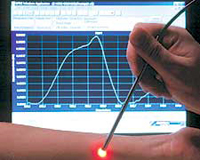
\includegraphics[width = 0.35\textwidth]{figures/DRS.jpg}	
%		\caption{Diffuse reflectance spectroscopy, Reflectance and absorption of light in skin}
%		\label{fig:DRS}
%		\end{figure}
%	
%	Multispectral imaging refers to a series of images captured at different wavebands across the electromagnetic spectrum. The wavebands can range from Ultra-Violet (UV) to InfraRed (IR). Using this advantage the multispectral image can contain more information beyond human eye capability. Such informations with respect to multilayer structure of the skin can be very useful. By using different wavelengths, the light is able to transfer in different depths and reveal various features related to skin layers.
%Opposed to standard colour camera which is able to capture the skin image in three channel of (red, green, blue), multispectral imaging system acquires a sequence of gray level images at different wavelengths. This extended spectral capacity provides a high advantage in skin imaging since it is reducing the effects of metameric mismatches, which may occur due to different illumination and variability of sensor spectral responses \cite{jolivot2011developpement}.
%	The spectral device of multispectral system, can be placed either in incident path, or in detection path. In either way, the main motivation is to go beyond the limited red, green and blue colour information which are available by other imaging techniques. This technique combines the advantage of both spectrophotometer and digital camera. The MS system acquire three dimensional data, the spatial information in 2 dimension and a spectral information in third dimension. Such system provides the spectral information for each pixel in the image. 	
%	
%	
%	The MS imaging systems are further discussed in Chapter \ref{CH:MS}.
%
%
%%A new category, called HyperSpectral Imaging (HSI) system is currently investigated
%%by several research groups, mainly in microscopy [Ornberg et al., 1999] [Rothmann et al.,
%%1998] and also for in-vivo optical diagnosis [Vo-Dinh et al., 2004]. However limitations
%%of HSI are generally their complexity, cost and acquisition time [Balas et al., 2001] which
%%may be affected by camera displacement. MSI and HSI systems are different because
%%MSI systems generally involve 4 to 20 spectral bands when HSI systems are capable of
%%recording higher number of very narrow spectral bands (20 - 100) [Vo-Dinh et al., 2004];
%%hence the spectral resolution is higher for HSI.
%%Figures 2.21(a),2.21(b),2.21(c),2.21(d) are the decomposition into spectral bands of a
%%skin lesion. The figures provide the different spectral channels given respectively by the
%%eyes, a RGB camera, a MSI system and a HSI one. It highlights that the amount of
%%spectral information about skin lesions is gradually increased from digital colour camera
%%to HSI.
%%Most of MultiSpectral and HyperSpectral Imaging techniques require several exposures
%%to acquire a data cube. Therefore, the acquired data have to justify the extra-time/cost
%%in comparison to colour camera that acquires an image with a single exposure. When
%%spectral acquisition is preformed successively, stacking together spectral data acquired
%%even at short period of time might be affected by motion artefact. The justification is
%%provided by the increased amount of information available about the skin reflectance not
%%seen by the human eye.
%%Once a spectral image is acquired, several mathematical approaches ranging from spa-
%%tial to spectral can be used to analyse the data. The analysis can be performed on the
%%spectral image (corrected after calibration) or this image can be transformed from a spec-
%%tral image to a reflectance cube. The state of the art of skin analysis techniques are
%%presented in chapter 4. In the following chapter, we present our own imaging system for
%%dermatological applications.
%
%	
%	\subsection{Dermoscopy}
%	Dermoscopy initially referrers to a non-invasive surface microscopy technique which is used for in vivo examination of epidermis and papillary dermis\cite{soyer1987early}. Dermoscopy brings new morphological criteria for differentiation of melanoma compared to other melanocytic and non-melanocytic pigmented skin lesions. A dermoscope can be seen similar to a magnifying lens which might contains extra features such as a built-in illumination system, a higher magnification and polarized filters. The principle of dermoscopy is transillumination which throws a strong light through an organ or part of skin as a mean of diagnosis of a skin area. This technique uses the fact that light incident on skin experiences reflection, refraction, diffraction and absorption and the physical properties of the skin are the source of these phenomena. Dermoscopy allows visualization of subsurface structures of dermis and papillary dermis which is not apparent to the unequipped eye by elimination the skin reflections from detected information. 
% Elimination of skin reflections can be achieved by applying linkage fluid to the skin, or using polarized light and polarized filters. \\
% Depending on the source light dermoscopy can be divided into two category, conventional Non-Polarized light contact dermoscopy (NPD), Polarized light dermoscopy (PD). The former category further can be divided into two group of polarized contact dermoscopy (PCD) or non-contact polarized dermoscopy(PNCD). Figure \ref{fig:NPD-PD} shows skin lesion images acquired with NPD and PD and Fig. \ref{fig:NPD-PD-NCPD} compares images of melanoma lesion via clinical imaging, non polarized dermoscopy, polarized light contact dermoscopy and polarized light non-contact dermoscopy \cite{Benvenuto-Andrade2007}
%
%	\begin{figure}
%	\centering
%	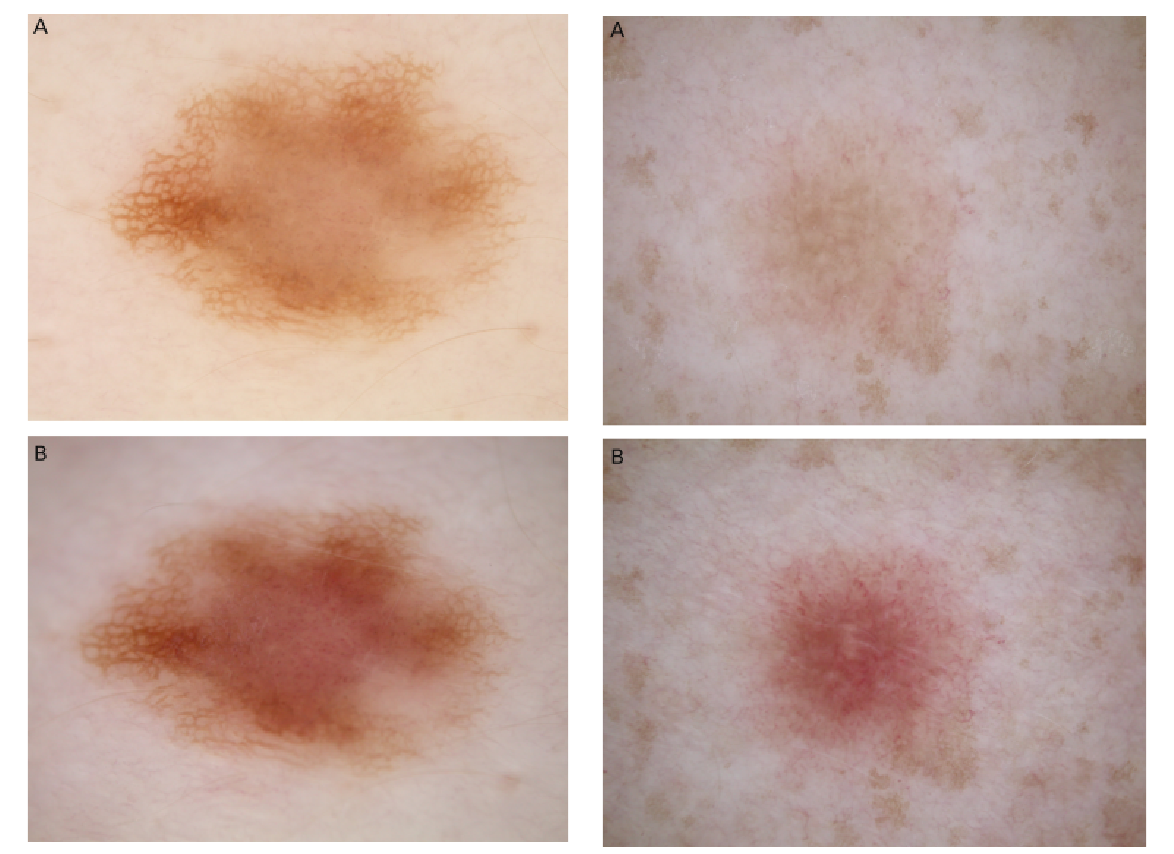
\includegraphics[width = 0.6\textwidth]{figures/NPD_PD_01.png}	
%	\caption{The images of atypical nevus (left) and MM lesion (right) with non polarized dermoscope(NPD, first row) and polarized dermoscope(PD, second row)\cite{wang2008differences}}
%	\label{fig:NPD-PD}
%	\end{figure}	 
%	
%	\begin{figure}
%	\centering
%	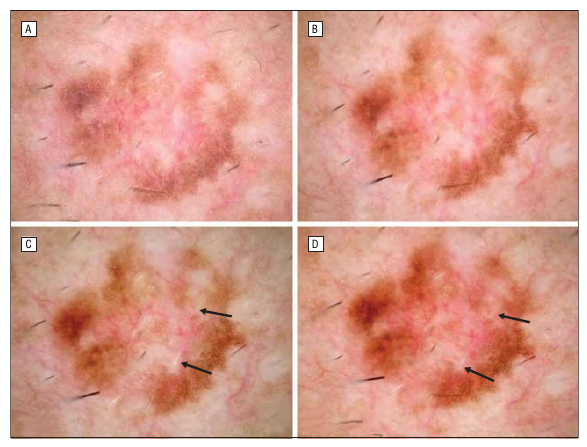
\includegraphics[width = 0.6\textwidth]{figures/Clinic_NPD_PD_NCPD.png}	
%	\caption{(A) A melanoma shown by clinical photography, (B) nonpolarized light contact dermoscopy (NPD),
%(C) polarized light contact dermoscopy, (D) and polarized light noncontact dermoscopy. This melanoma had evidence of regression (fibrosis) on histopathological examination. Shiny-white streaklike areas within the melanoma (arrows in C and D), believed to represent fibrosis, are visiblein order to obtain full 2D image of any sample in short time.  under polarized but not NPD\cite{Benvenuto-Andrade2007}}
%	\label{fig:NPD-PD-NCPD}
%	\end{figure}	 
%	
%	
%The NPD dermoscopy is also referred as \textit{in vivo cataneous surface microscopy}, \textit{magnified oil immersion  diascopy} and most commonly \textit{epiluminescence microscopy (ELM)}. This technique gets use of a hand held incident light, magnifying device (microscope) and immersion liquid in order to provide translucent surface of the skin and eliminates the reflections. The goal is to eliminate the surface scattering by minimizing the change of refractive index at skin/air interface. Immersion liquids such as oil, water or alcohol, has a refraction index relatively similar to skin and have been applied on skin surface prior to imaging. The contact between the skin and the glass interface of microscope is necessary in this case. The refractive of the glass is also very similar to the skin. 
%The whole system, makes the stratum corneum of the skin translucent and reduces the amount of reflection at the skin surface. 
%
%	\begin{figure}[h]
%	\centering
%	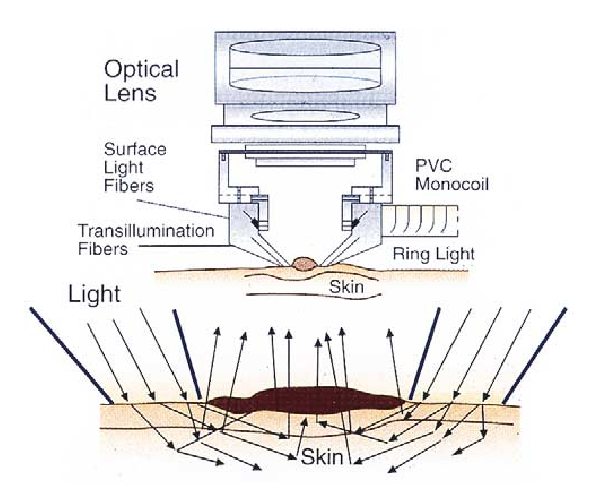
\includegraphics[width = 0.5\textwidth]{figures/Nevoscope.png}	
%	\caption{Dermoscopy functions by transillumination oflesion (Nevoscope)\cite{Marghoob2003}}
%	\label{fig:Nevoscope}
%	\end{figure}
%
%The PD dermoscope consists of polarized light and two cross polarized filters in order to block the reflected lights and passing the scattered lights with in skin through the lens. One horizontal linear polarized filter is mounted in front of the source light, while the other filter, vertical linear polarized filter, is mounted in front of the detector. This allows for almost complete elimination of the reflection. 
%Although the direct contact for the NPD and PCD is necessary, for PNCD there is no need for liquid interface neither direct contact.
%
%
%Another imaging techniques, related to dermoscopy is the transilumination technology (TLM). This technique is patented and used only for a device called \textit{Nevoscope} (see Fig.\ref{fig:Nevoscope}) In this technique, the light is directed to the skin in such a way that allows the backscattered light illuminates the lesion from with in \cite{Patwardhan2003,patwardhan2004multi,patwardhan2005monte}.\\
%
%
%
%	\section{Skin Optical Properties}
%	 
%Skin has two main optical properties which are absorption and scattering. If we assume an incident light with close incidence angel to normal, only \% 5 of the incident light is directly reflected at the surface, while the rest of the light is entered in the skin and goes through absorption and scattering phenomena. This pathway is also shown in Fig. \ref{fig:pathwayofLight}
%	\begin{figure}[h]
%	\centering
%	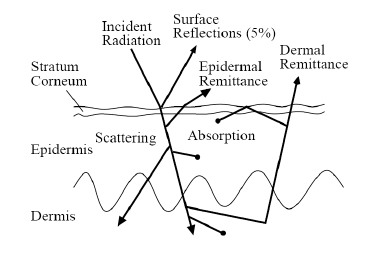
\includegraphics[width = 0.45\textwidth]{figures/PWofLightinSkin.png}	
%	\caption{Pathway of incident light in skin \cite{storring2000estimation}}
%	\label{fig:pathwayofLight}
%	\end{figure}
%
%	Melanin and haemoglobin are the two important chromophores which play important part in appearance of normal skin and are responsible for absorbing the light. These chromophores strongly absorb light in the ultraviolet (UV) and visible ranges and have low absorption rate near-infrared range.	 
%%Melanin is the major chromophore of the epidermis which occupies the top 50-100 \micro\meter, with the exception to superior layers of epidermis. Melanin is produced by melanosomes when exposed with UV light and is divided into two  types eumelanin and pheomelanin. Eumelanin has black/brown colour while pheomelanin has red/yellow colour. Concentration of this components are different between individuals, leading to different colour skins. 
%
%%Haemoglobin is a chromophore of red colour found in the microvascular network of the dermis, typically 100-500 \micro\meter below the skin surface. This chromophore caries oxygen through vessels and capillaries. This chromophore accordingly is called oxy-haemoglobin while it contains oxygen and deoxy-haemoglobin otherwise.
%	The absorption phenomenon correspond to the energy attenuation of a photon due to the absorption of a particle or a group of particles. The absorption coefficient of a layer is a function of the molar concentration and the absorption coefficient of the molecules presented in that layer. Meglinski et al \cite{meglinski2002quantitative} had defined the absorption coefficients of the single layer by set of equations as follows:
%	\begin{equation}
%	\footnotesize	
%	\mu_{a}(\lambda)= \sum_{i=1}^{m}\big(\mu_{a}^{(i)}(\lambda)C_{i}\prod_{j=1}^{i-1}(1-C_{j})\big)+\mu^{(0)}(\lambda)\prod_{j=1}^{i-1}(1-C_{j})
%	\label{Eq:AbsorptionCoefficient}
%	\end{equation}
%
%	\begin{equation}
%	\footnotesize
%	\begin{split}
%	\mu_{a}^{layer}(\lambda)= (1-S) \gamma C_{blood} \mu_{a}^{Hb}(\lambda) + 
%	S\gamma C_{blood}\mu_{a}^{HbO_{2}}(\lambda) + \\
%	(1-\gamma C_{blood})C_{H_{2}O} \mu_{a}^{H_{2}O}(\lambda) + (1-\gamma C_{blood})(1-C_{H_{2}O})\mu_{a}^{(0)}(\lambda) 
%	 \end{split}
%     \label{Eq:AbsorptionCoefficientLayer}
%	 \end{equation}
%	 \begin{subequations}
%	\begin{center}
%	\begin{align}
%	\mu_{a}^{(0)}(\lambda)= 7.84 \times 10^{7} \times \lambda ^{-3.255}\\
%	\gamma = F_{Hb} F_{RBC} H_{t}	
%	\end{align}
%	\end{center}
%	\label{Eq:AbsorptionCoefficientmuandgamma}
%	\end{subequations}	 
%
%	In the above equations, $C_{i}$ is the volume fraction of the $i^{th}$ molecule, $m$ is the total number of molecules in the layer, $\mu_{a}^{(i)}$ is the absorption coefficient of the $i^{th}$ absorber and $\mu^{(0)}$ is the absorption coefficient of the medium without absorber. $\mu_{a}^{H_{2}O}$, $\mu_{a}^{HbO_{2}}$ and $\mu_{a}^{Hb}$ are the absorption coefficients of water, oxy and deoxy haemoglobin respectively and their values over the VIS and NIR spectrum (400–1100 nm) 
%are shown in Fig.\ref{fig:waterabsorptioninSkin}. $C_{blood}$ and $C_{H_{2}O}$ are the layer volume fractions of blood and water (see Table \ref{T:MeglinskiTable}).  $S$ is the oxygen saturation in blood and is assumed to be constant at 0.6. $\gamma$ is the total fractions of haemoglobin in blood and can be calculated using three parameters of $F_{Hb}$ (volume fraction of haemoglobin in an erythrocyte),  $F_{RBC}$ (volume fraction of erythrocytes in the total volume
%of all blood cells) and $H_{t}$ (the haematocrit). The values of these parameters were considered constant such as: 0.25, 0.99 and 0.45 respectively. \\
%	
%	\begin{table}
%	\caption{The parameters used in the skin model defined by \cite{meglinski2002quantitative}}
%	\begin{center}
%	\footnotesize
%	\begin{tabular}{ c c c c c c c}
%	\hline 
%	k &  $\#$ Layers & $C_{blood}$ & $C_{H_{2}O}$ & $\mu_{s}$($mm^{-1}$) & g & n \\
%	\hline 
%	1 & Stratum corneum & 0 & 0.05 & 100 & 0.86 & 1.5 \\
%	2 & Living epidermis & 0 & 0.2 & 45 & 0.8 & 1.34 \\
%	3 & Papillary dermis & 0.04 & 0.5 & 30 & 0.9 & 1.4 \\ 
%	4 & Upper blood net dermis & 0.3 & 0.6 & 35 & 0.95 & 1.39 \\ 
%	5 & Reticular dermis & 0.04 & 0.7 & 25 & 0.8 & 1.4 \\
%	6 & Deep Blood net dermis & 0.1 & 0.7 & 30 & 0.95 & 1.38 \\
%	7 & Subcutaneous fat & 0.05 & 0.7 & 5 & 0.75 & 1.4 \\
%	\hline 	  
%	\end{tabular}
%    \end{center}
%	\label{T:MeglinskiTable}	
%	\end{table}
%	
%	\begin{figure}
%	\centering 
%	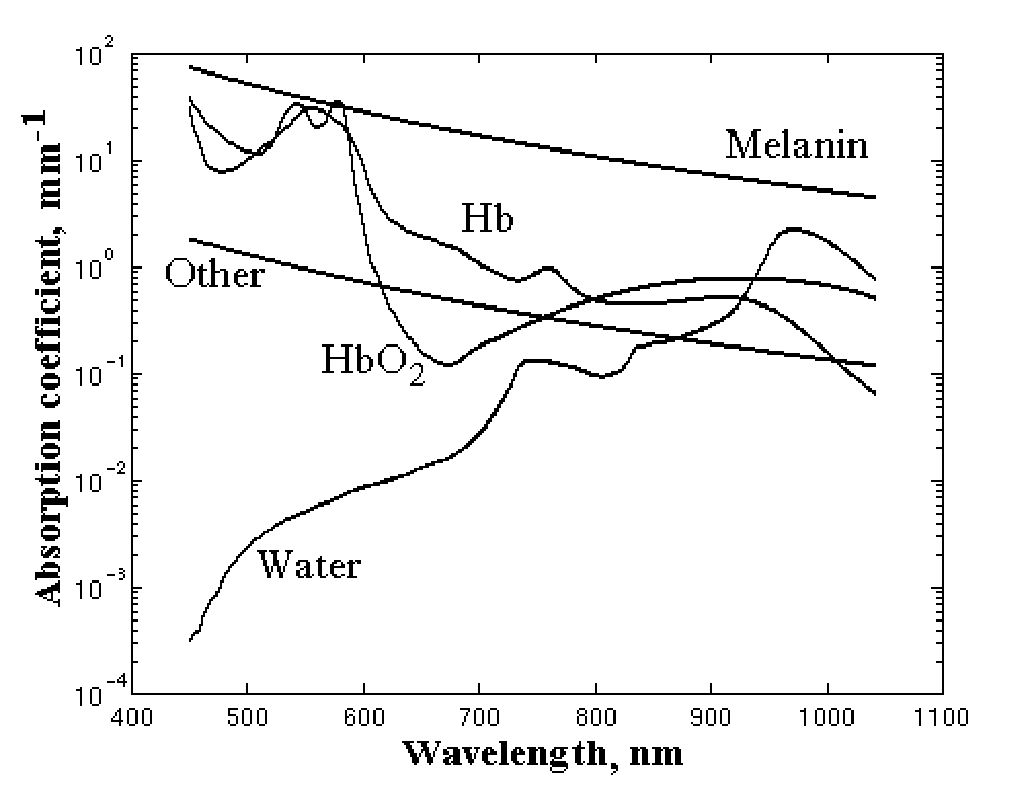
\includegraphics[width = 0.6\textwidth]{figures/AbsorptionCoeff.png}	
%	\caption{The absorption coefficients of oxy, deoxyhaemoglobin and water as a function of
%wavelength \cite{jacques1996origins}}
%	\label{fig:waterabsorptioninSkin}
%	\end{figure}
%	
%	
%	Jacques et al \cite{jacques1996origins} also defined the dermis and epidermis absorption coefficients in a less complicated form (see Eq.\ref{Eq:Abs-Jac}) as follows: 
%	
%	\begin{subequations}	
%	\begin{align}	
%	\mu_{a,epi} =f_{mel}.\mu_{a,mel}+ (1-f_{mel})-\mu_{a,skin}\\
%	\mu_{a,der} = f_{blood}.\mu_{a,blood}+(1-f_{blood}).\mu_{a,skin}\\
%	\mu_{a,mel} = 6.6 \times 10^{11}\lambda ^{-3.33}\\
%	\mu_{a,skin} = 0.244 + 85.3 \exp(-(\frac{\lambda -154}{66.2})) 
%	\end{align}
%	\label{Eq:Abs-Jac}	
%	\end{subequations}
%	
%	In equation \ref{Eq:Abs-Jac} $f_{mel}$ is the volume fraction of melanosomes, $f_{blood}$ is the blood fraction  and $\mu_{a,blood}$, $\mu_{a,mel}$, $\mu_{a,skin}$ are the absorption coefficients of haemoglobin, single melanosome, and skin layer without any chromophores, respectively. \\
%
%	Scattering is raised from fibres, cell and cellular organelles. Multiple scattering of light incident is expected after interacting with skin fibres. This phenomena will create reflectance spectrum which can be measured by considering the absorption and scattering properties of skin. Scattering is referred to a direction change of a wave after its interaction with one or several elements of the medium. Mie theory and Rayleigh are used to define this optical property for single particle or multiple particles respectively. Rayleigh scattering is observed in wavelengths below 650 \nano\meter, while Mie scattering is more effective above 650 \nano\meter. It was observed that epidermis and dermis have equal reduced scattering coefficient which is the result of Rayleigh and Mie scattering parameters. Figure \ref{fig:RayMieSkin} shows this relation. The Rayleigh and Mie scattering coefficients as well as dermis and epidermis are define as \cite{jacques1996origins}: 
%
%	\begin{subequations}
%	\begin{align}
%	\mu_{s, Rayleigh}(\lambda) = (2\times 10^{12})\lambda^{-4} \hspace{0.5 cm} [cm^{-1}]\\
%	\mu_{s, Mie}(\lambda) = (2\times 10^{5})\lambda^{-1.5} \hspace{0.5 cm} [cm^{-1}]\\
%	\mu'_{s, epidermis}(\lambda) = \mu'_{s, dermis}(\lambda) = \mu_{s, Rayleigh}(\lambda) + \mu_{s, Mie}(\lambda) 
%	\end{align}		
%	\label{Eq:SEpiDer}
%	\end{subequations}
%
%	\begin{figure}
%	\centering 
%	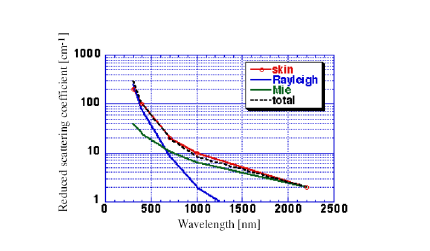
\includegraphics[width = 0.7\textwidth]{figures/RayleighMieSkin.png}	
%	\caption{Relation between reduced scattering coefficient, Mie scattering and Rayleigh scattering \cite{jacques1996origins}}
%	\label{fig:RayMieSkin}
%	\end{figure}
% Based on Fig.\ref{fig:RayMieSkin}, it is evidence that incident lights with longer wavelength could reach deeper in the skin. A complete survey on skin behaviour, properties and its appearance modelling is represented by \cite{igarashi2007appearance}. 
%	
%\section{Light Propagation Models in Skin}
%
%Modelling the propagation of light in skin is a difficult and complex task, as a result several models have been proposed so far. 
%Incident light in interaction with skin, is either reflected, refracted, scattered or absorbed. The two terms reflection and refraction are very close and simply can be confused. It should be considered that reflection occurs when waves bounce off a surface and travel onward with new angle and could be specular or diffuse. On the other hand refraction occurs when the light speed is changing as well as its direction. 
%The reflected light from a surface is generally modelled by Dichromatic Reflection Model \cite{klinker1990physical}. This model describes total reflection as a combination of surface reflection (specular reflection, \% 5 for skin medium) and body reflection, which is reflected from the body of the medium (diffuse, \% 95 in the case of skin).  
%
%	\begin{equation}
%	 L_{Ref} = L_{Ref, Sur} + L_{Ref, Body}
%	 \label{eq:LRef}
%	\end{equation}
%
%Considering different cases of light interaction with skin, and knowing the absorption and scattering coefficients of different skin layers and components, a propagation model can be modelled. Several models have been proposed including, the radiative transfer equation, monte carlo simulation, kubelka-monk model and modified bear lambert law. These models are discussed in the next section.  
%
%\subsection{Radiative Transfer Equation Model}
%
%The Radiative Transfer Equation (RTE) is referred to the mechanism of exchanging energy between atmosphere and underlying surface and between different layers of atmosphere. This model describes how the physical properties of the material are coupled to the measured spectrum. This model is commonly employed to model light propagation in scattering media. It is also used for modelling neutron propagation in nuclear reactor and propagation of gas in the atmosphere. 
%
%In this model, the light is expressed in terms of its average energy after interacting with media and multiple scattering and it is defined in terms of intensity instead of electromagnetic field (see Eq.\ref{eq:LightAFSca})
%	\begin{equation}
%	dP = I(r,\hat{s},t)d\Omega da 
%	\label{eq:LightAFSca}
%	\end{equation}
%In the above equation, $dP$ is the light power at time $t$ which is propagating along direction $r$ to meet the particle at section $da$. The section $da$ is considered in a cone with solid angel $d\Omega$, which is oriented along the unit vector $\hat{s}$. This vector is normal to the surface area of $da$. $I(r,\hat{s},t)$ is the light power (quantity of photon) per unit area per unit solid angle. Equation \ref{eq:LightAFSca} represents the light energy in terms of geometry, however this equation can be represented based on scattering ($\mu_{s}$) and absorption ($\mu_{a}$) coefficients of the media and phase function as well.
%
%RTE model considers that only one type of particle is responsible for the scattering and absorption and the phase function is approximated by the Henyey Greenstein function. This model is considered as the most correct equation for representing the propagation of light in skin, however due to its complexity its direct impact had been rare in previous research. 
%Radiative transfer equation is defined using transport equations such as Boltzmann equation. In this formulation, light propagation is considered as a photon flux which can be absorbed or scattered by the biological medium. 
%	\begin{equation}
%	s.\vec{\bigtriangledown}(r,\hat s ) = -(\mu_{a}+\mu_{s})I(r,\hat s)+ \frac{\mu_{a}+\mu_{s}}{4\pi}\int_{4\pi} p(\hat s,\hat s')I(r,\hat s )d\Omega'
%	\label{Eq:Boltzmann}
%	\end{equation}		
%	
%RTE due to its integral differentiation nature tends to be rather complex and often intractable without exact analytical solutions. Although efficient numerical method could be crucial, approximation analytical methods are available, such as transfer matrix method, singular eigenfunction method, perturbation method and etc.
%
%Besides these methods several numerical techniques also have been used such as Monte Carlo method which is described in the next section. 
%
%\subsection{Monte Carlo Method}
%Monte Carlo (MC) methods are stochastic techniques. These methods take use of random variables and probability statistics to investigates the problems. These methods are useful to find numerical solutions to some problems which are analytically impossible or very complicated to solve. Monte Carlo method was first developed by Metropolis and Ulam \cite{metropolis1949monte} to simulate physical processes using a stochastic model. MC methods are used in different fields from economic, nuclear physics to regulating the flow of traffic. Monte Carlo is not represented by a specific technique and the term is applied to a wide range of techniques that can be applied. Although these techniques could be different , they all should follow the certain pattern:  
%
%	\begin{itemize}
%	\item A range of possible inputs are introduced to the system
%	\item A set of random variables are produced by considering the introduced input ranges. 
%	\item A series of mathematics calculations and statistics are performed using the random variables and inputs	
%	\item The computed results of each calculation is integrated in the final answer
%	\end{itemize}
%
%%%Numerical methods that are known as Monte Carlo methods can be loosely described as statistical simulation methods, where statistical simulation is defined in quite general terms to be any method that utilizes sequences of random variables to perform the simulation.	Accordingly all the MC methods rely on a good random variables and by simulating more data, they gradually converge to a better estimation. 
%
%Wang and Jacques et al. \cite{wang1992monte} introduced the earlier formulation of MC methods for multi-layered tissues. Figure \ref{fig:MC-Jacques} shows how they used their simulation to model the propagation of a photon through a homogeneous multi-layered medium (MCML).
%	\begin{figure}[h]
%	\centering 
%	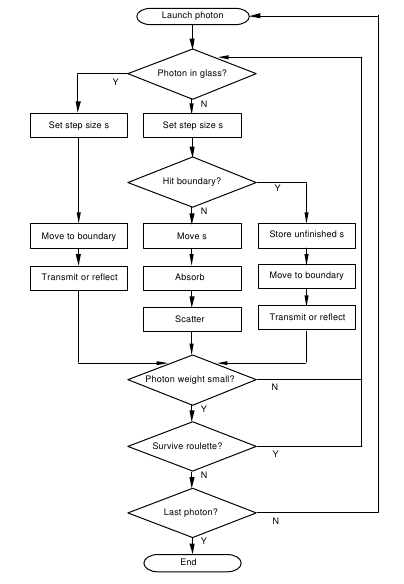
\includegraphics[width = 0.7\textwidth]{figures/MCMLFelowChart.png}	
%	\caption{Felow chart of MC method for multi-layered tissue \cite{wang1992monte}}
%	\label{fig:MC-Jacques}
%	\end{figure} 
%	
%Their approach later was used by \cite{tsumura2001mapping} for modelling the skin reflectance and mapping the skin pigmentation. The application of MC methods for modelling the light propagation through skin can be found in several articles \cite{meglinski2003computer, igarashi2007appearance}.
%
%The MC simulations statistically computes the optical pathway of each photon, repeatedly with many iterations in order to find accurate results. Assuming that the photon is injected into a scattering medium, MC methods estimates the optical photon paths in an iterative manner based on parameters such as $\mu_{s}$ and $\mu_{a}$ and the phase function. This method can be computationally expensive, considering numerous iterations (often in the order of millions) are required for accurate results. Another disadvantage of the method is the noise introduced by the stochastic approach. Due to this matters, analytical methods might be more preferable, although they require more assumptions. 
%
%%%We have simulated diffuse reflectance spectra of skin by assuming a
%%%wavelength-independent scattering coefficient for the different skin tissues and
%%%using the known wavelength dependence of the absorption coefficient of oxy-
%%%and deoxyhaemoglobin and water. A stochastic Monte Carlo method is used
%%%to convert the wavelength-dependent absorption coefficient and wavelength-
%%%independent scattering coefficient into reflected intensity. The absorption
%%%properties of skin tissues in the visible and near-infrared spectral regions
%%%are estimated by taking into account the spatial distribution of blood vessels,
%%%water and melanin content within distinct anatomical layers. The geometrical
%%%peculiarities of skin histological structure, degree of blood oxygenation and the
%%%haematocrit index are also taken into account. We demonstrate that when the
%%%model is supplied with reasonable physical and structural parameters of skin,
%%%the results of the simulation agree reasonably well with the results of in vivo
%%%measurements of skin spectra.
%%%
%%%
%%%The reflectance spectra of the human skin in visible and near-infrared (NIR) spectral region have been calculated
%%%using the Monte Carlo technique, and the specular and internal reflection on the medium surface is taken into account.
%%%Skin is represented as a complex inhomogeneous multi-layered highly scattering and absorbing medium. The model
%%%takes into account variations in spatial distribution of blood, index of blood oxygen saturation, volume fraction of
%%%water and chromophores content. The simulation of the skin tissues optical properties and skin reflectance spectra are
%%%discussed. Comparison of the results of simulation and in vivo experimental results are given.
%
%\subsection{Kubelka Munk Model}
%The Kubelka-Munk (K-M) theory is one of the most popular and simplest approaches for computing the light transport in highly scattering medium. This theory was first developed by \cite{kubelka1931article}. In this article Kubelka and Munk introduced their theory based on the relationship between the scattering and absorption coefficients of layers of paint and its overall reflectance. K-M theory describes the radiation transfer in diffuse scattering media, by applying energy transport equations. K-M theory allows the quantitative studies of absorption, scattering and luminescence in diffuse scattering media and was used by different groups to skin analysis \cite{krishnaswamy2004biophysically,igarashi2007appearance,doi2003spectral,vyas2012computational,jolivot2011developpement}. 
%K-M model has an analytical approach and is able to determine rapidly the skin optical parameters, using inversion approaches. 
%The K-M model measures reflectance and transmittance of incident light in a scattering media, by relating the medium optical properties and K-M equations. This model considers three ways of interaction between incident light and the medium (reflection, absorption and transmission) and considers that the incident light flux is dividing into two fluxes ($I$, $J$), which are passing in two opposite direction in a medium (see Fig. \ref{fig:KMfig}). The energy variation of these fluxes over an infinitely small distance ($d$) are defined by the K-M equations:
%	\begin{subequations}
%	\small
%	\begin{align}
%	dI = (-kI-sI +sJ)dx\\
%	-dJ = (-kJ -sJ+sI)dx
%	\end{align}
%	\label{Eq:KMEq}
%	\end{subequations} 
%	
%	\begin{figure}[h]
%	\centering 
%	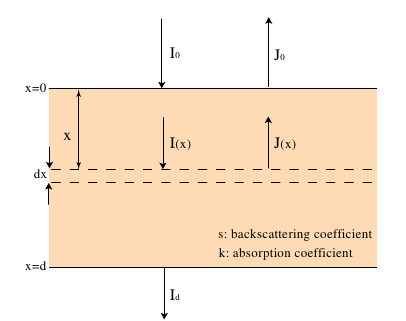
\includegraphics[width = 0.6\textwidth]{figures/KMfig.png}	
%	\caption{Illustration of light transport in an optical medium modele based on Kubelka–Munk theory. $I$ and $J$ illustrate diffuse fluxes travelling in the forward and backward directions,respectively. $s$ and $k$ are the backscattering and absorption coefficients of the medium,respectively and d is the sample thickness. \cite{igarashi2007appearance}}
%	\label{fig:KMfig}
%	\end{figure} 
%	
%Where $I$ is the light intensity inside the sample going downward (transmitted) and $J$ is the light intensity inside the sample going upward (backscattered). $s$ and $k$ are the scattering and absorption coefficients per unit thickness respectively and $x$ is the distance of the interaction. 
%
%The reflectance ($\frac{J_{0}}{I_{0}}$) and transmittance ($\frac{I_{d}}{I_{0}}$) of the medium are related to the scattering and absorption coefficients as :
%
%	
%	\begin{subequations}
%	\small
%	\begin{align}
%	R = \frac{(1-\beta ^{2})(exp(Kd)-exp(-Kd))}{(1+\beta) ^{2}exp(Kd)-(1-\beta) ^{2}exp(-Kd)}\\
%	T = \frac{4\beta} {(1+\beta)^{2}exp(Kd)-(1-\beta)^{2} exp(-Kd))}\\  
%	K = \sqrt{k(k+2s)} \hspace{0.7cm},\hspace{0.7cm}  \beta = \sqrt{\frac{k}{k+2s}}
%	\end{align}
%	\label{eq:RTKB}
%	\end{subequations}
%
%
%Kubelka-Munk theory assumes that the sample possesses inhomogeneities, which are small compared to its thickness and incident radiation is diffused and the regular reflection at the boundaries can be neglected \cite{jolivot2011developpement}. Due to these assumptions, it causes false estimations in certain cases, for instance this model overestimates the radiance of scattered light in a medium with high albedo (strongly anisotropic scattering medium), such as superficial area of the skin \cite{igarashi2007appearance}. This method can not predict the spatial distribution of light due to scattering as well, since only two scattering direction of light is considered. 
%However due to its simplicity, speed and its extension to NIR \cite{cotton1997noninvasive}, it has been used by different groups for modelling the light transport through the skin and retrieving internal parameters such as epidermal melanin, dermal blood, papillary dermal thickness \cite{cotton1997noninvasive,jolivot2011developpement}



%%%The scattering and absorption coefficient can be written in terms of reflection and transmittance parameters as it is stated by Eq. \ref{Eq:SK-RT}
%%%	
%%%	\begin{subequations}
%%%	\small
%%%%	\begin{center}
%%%	\begin{align}
%%%	\frac{S}{K} = \frac{1+R^{2}-T^{2}}{2R}-1\\
%%%	S.t, \hspace{0.1cm} layer_{thickness} \gg 0, \hspace{0.1cm} T = 0	,  \hspace{1cm} \frac{S}{K} = \frac{(R-1)^{2}}{2R} 
%%%	\end{align}
%%%%	\end{center}
%%%	\label{Eq:SK-RT}
%%%	\end{subequations} 
%%%
%%%
%%%The equations \ref{Eq:SK-RT} can be extended for two and more $n$ layers. The total remittance $R_{1,2}$ and transmittance $T_{1,2}$ for two layers which is based on the reflectance and transmittance of each layer is stated in the following equation: 
%%% 	
%%%	\begin{subequations}
%%%	\small
%%%	%\begin{center}
%%%	\begin{align}
%%%	R_{1,2} =R_{1} + T_{1}T_{2}R_{2}(1+R_{1}R_{2} + R_{1}^{2}R_{2}^{2}+\ldots) = R_{1} + \frac{T_{1}^{2}R_{2}}{1-R{1}R_{2}}\\
%%%	T_{1,2} = T_{1}T_{2}(1+ R_{1}R_{2} + R_{1}^{2}R_{2}^{2}+\ldots) = \frac{T_{1}T_{2}}{1-R_{1}R_{2}}
%%%	\end{align}
%%%	%\end{center}
%%%	\label{Eq:TR2}
%%%	\end{subequations} 
%%%
%%%Equation \ref{Eq:TR2} can be extended for n layers such as: 
%%%	\begin{subequations}
%%%	\small
%%%	%\begin{center}
%%%	\begin{align}
%%%	R_{1,2,\ldots n} =R_{1,2,\ldots n-1} + \frac{T_{1,2,\ldots ,n-1}^{2}R_{n}}{1-R_{1,2,\ldots, n-1}R_{n}}\\
%%%	T_{1,2,\ldots n} = \frac{T_{1,2,\ldots n-1}T_{n}}{1-R_{1,2,\ldots, n-1}R_{n}}
%%%	\end{align}
%%%	%\end{center}
%%%	\label{Eq:TRn}
%%%	\end{subequations} 

%\subsection{Modified Beer-Lambert Law model}
%
%Beer-Lambert law is modelling the light transport in an optical medium, assuming the scattering is small and absorption effects is much greater than scattering. In this case the incident light goes directly into the medium and gets attenuated exponentially due to absorption \cite{igarashi2007appearance}. This law is written as: 
%	\begin{equation}
%	 L = (1-R_{F})E exp(-\mu_{t}d)
%	\label{eq:BL}
%	\end{equation}
%where $L$ is the radiance, $E$ is incident radiance, $R_{F}$ is the coefficient of Fresnel reflectance for normal light incidence and d is the thickness of the optical medium. This model works well when absorption coefficient is at least 10 times greater than scattering coefficient which is the condition when skin is illuminated in ultraviolet and far infra-red light and does not hold for the visible and near infra-red illumination. Since this model is invalid for modelling the light transport in skin, the modified Beer-Lambert law was proposed \cite{igarashi2007appearance}.
%
%The modified Beer-Lambert law is considering highly scattering medium and since the optical path length in a highly scattering medium is not the same as the medium thickness it modified the original formula by considering the mean path length of the scattered light $d(\lambda)$, 
%	\begin{equation}
%	 L = (1-R_{F})E(\lambda) exp(-\mu_{a}d(\lambda))
%	\label{eq:BL}
%	\end{equation}
%
%The modified Beer-Lambert law was used by \cite{meglinski2003computer,shimada2001melanin,tsumura2003image} in order to model the light transport in skin. In \cite{meglinski2003computer} it was shown how modified Beer-Lambert law uses linear equation to relate the tissue attenuation with its absorption coefficient. In this relation, $\rho$ is the space between the source and the detector and $\sigma$ is the scaling factor, $G$ is an offset term determining either the tissue probe geometry or the scattering coefficient. This equation can be extended for N chromophores as well (see Eq.\ref{Eq-BLA}.b) and the properties of theses chromophores can be obtained by measuring $A$ with a minimum N+3 wavelengths and using multi-linear regression. In this equation, $\mu_{a}$ is represented as sum of absorption coefficient for each choromophore, which is determined by the concentration ($C_{i}$) and specific absorption coefficient ($\epsilon_{i}$) of each choromophore.  
%
%	\begin{subequations}
%	\begin{align}
%	 A = -ln \frac{I}{I_{0}} = \mu_{a} \sigma_{\rho} + G\\
%	 A = a + b\lambda + \sum_{i=1}^{N} C_{i}\epsilon_{i}(\lambda)
%	 \end{align}
%	\label{Eq-BLA}
%	\end{subequations}



%%%%%%%%%%%%%%%%%%%%%%%%%%%%%%%%%%%%%%%%%%%%%%%%%%%%%%%%%%%%%%%%%%%%%%%%%%%%%%
%%% CHAPTER 2
%%%%%%%%%%%%%%%%%%%%%%%%%%%%%%%%%%%%%%%%%%%%%%%%%%%%%%%%%%%%%%%%%%%%%%%%%%%%%
%%\chapter{Multispectral Imaging}
%%\label{CH:MS}
%%
%%\section{Introduction}
%%The series of images from one scene acquired at different waveband are called multispectral image. This technique provides the means to extract additional information from the scene and it has been used in a wide variety of applications, such as remote sensing, biomedical imaging, target recognition and tracking. In the case of skin, variety of information can be extracted from different layers of skin as they exposed to various wavelengths of light. Moreover based on attainable depth for each wavelength multiple layers of skin will be visible for further analysis. This property is of great interest for evaluation of pigmented lesions. Opposed to a standard colour camera which provides three color channel (Red, green, blue) of the skin, the multispectral system acquire gray level images at each wavelength. The set of grey level images at different wavelengths provides external spectral information about the object and decreases the metameric mismatches that might occurs with standard color or grey cameras under different illumination. \\
%%
%%The data attained by the MS system consist of three dimensions, two spatial dimensions, and one spectral dimension.The MS system can collect the data either by spatial scanning or spectral scanning. 
%%
%%\subsection{Spectral Scanning}
%%In spectral scanning the images are acquired for each spectral band. This model is defined by a set of spectral imaging optics (filters) and a camera. Different wavelengths can be achieved by fixed or tunable filters. \\
%%
%%Fixed filters allow for easy and considerably cheap development of multispectral system. Desired wavelengths are achieved by placing bandpass filters in the optical path. Most commonly the bandpass filters are mounted on a wheel and their rotation are synchronized with the camera acquisition. Although fixed filters have the advantage of low cost equipment and large selection field, they are not flexible in terms of filter specifications and also the number of filters are restricted to the mechanical size of the system. Besides these restriction, perhaps due to the availability and cheap cost, filter wheel was used by several researchers, in order to build the multispectral system \cite{yamaguchi2005multispectral,marchesini1994telespectrophotometry,gutkowicz2000precision,jolivot2011developpement}.\\
%%
%%
%%Tunable filters can also be used for spectral scanning. These filters are able to continuously shift the spectral transmission band along the electromagnetic spectrum at any wavelength ($\lambda$) within their defined spectral capability range. They can modify the transmission wavelength by electrically tuning their spectral waveband. 
%%
%%The Liquid Crystal Tunable Filter (LCTF) and Acousto Optic Tunable Filter (AOTF) are two types of tunable filters. Both filters are polarized sensitive. This means that their transmission power is decreased by at least half. 
%%
%%The liquid crystal tunable filter (LCTF) consist of liquid crystal layers. This optical device electrically controls each liquid crystal for transmitting different wavebands. Each LCTF have different stages. Each stage is composed of two parallel polarizer with one birefringence retarder and a liquid crystal in the middle (see Fig. \ref{fig:LCTF}). Every stage produces a sinusoidal transmission curve with specific frequency. Combination of all the sinusoidal curves as a result of individual stages, will lead to a constructive interference and one curve with overall transmission characteristics at one wavelength. The LCTF tunes the wavelength of the bandpass filter by controlling the wavelength which constructive interference occurs. This task is done by applying a voltage across the birefringence at each stage. 
%%
%%	\begin{figure}
%%    \subfloat[Liquid crystal tunable filter]{    
%%    \includegraphics[width=0.45\textwidth]{figures/LCTF.png}
%%    \label{fig:LCTF}
%%    }
%%	\subfloat[Acousto optic tunable filter]{
%%	\includegraphics[width=0.42\textwidth]{figures/ALTF.png}
%%	\label{fig:AOTF}
%%	}
%%	\end{figure}	 
%%
%%Acousto optic tunable filters (AOTF) are another type of tunable filters. These filters are based on interaction between a crystal lattice and an acoustic wave, which are controlled electrically. Changes in the acoustic frequency will modify the diffraction properties of the crystal lattice and will tune the wavelength. When acoustic wave propagate through the crystal, it creates a grating. The modification of the acoustic wave alter the density and local refraction index of the crystal. The whole system performs as a diffraction grating and filter out one wavelength depending on the acousto wave frequency. 
%%
%%Opposed to LCTF, AOTF has the advantage of rapid tuning (microseconds compare to milliseconds) and broader wavelength ranges. However since they rely on the acoustic wave effects for changing and shifting the frequency, their image quality is considerably poor. The AOTF is also able to generate multiple bandpass at a time while LCTF can generate single bandpass. Despite AOTF, LCTF are able to provide better image quality and due to their lightness and low power consumption, they have been used for remote sensing application, space and airborne imaging. LCTF was used in \cite{shi2007multispectral,kuzmina2010multispectral} for construction of multispectral system. \\
%%%In \cite{shi2007multispectral}, the selected LCTF has an 8 \nano\meter bandwidth at the selected wavelength and the transmission of \%25 - \%35 for the range of wavelength from 480 to 720 \nano\meter \cite{shi2007multispectral}.\\
%%
%%In comparison to fixed filter, tunable filters are not affected by mechanical constraints, image shift, speed limitation and vibration. However since tunable filters are polarized dependence, they have a weaker transmission and require a stronger illumination source to compensate the drawbacks. 
%%
%%	 
%%	\subsection{Spatial Scanning}
%%	Spatial scanning is the acquisition of spectral information along a spatial dimension, at a single time. This technique can used either single slit spectrometer or multi-slits spectrometer. A single slit system scans a spectrum through x-y spatial coordinates. Using this technique, the data cube is obtained after scanning the object in both x and y direction. A multi-slit technique scans a line and acquires an image onto a two dimensional camera (spatial information is projected to one axis and the spectral information along another one). The data cube in this case is obtained by scanning the area of interest which is perpendicular to the acquisition line. 	The acquisition time for both techniques are much longer than other methods and they require a motionless object during an acquisition \cite{burton2009spectral}.
%%	
%%	\section{Review on Multispectral Systems}	
%%
%%The application of multispectral imaging techniques was discovered first in environmental fields and remote sensing. However not far after, this technique was introduced to medical science. In medical application, multispectral systems have been used for endoscopy, skin spectroscopy and imaging. Related to skin imaging this method also has been used for finger prints identification in biometric field \cite{rowe2008multispectral}.\\
%%
%%The word endoscopy referees to looking inside body parts for medical diagnosis. The combination of multispectral and endoscopy with the aim to identify the cancerous regions can be found in literature. This combination is investigated for different cancers such as cervical \cite{anastasiadou2008polarimetric}, colon \cite{joshi2012targeted}, ear \cite{leitner2012multi} and stomach. \\
%%
%%There are researches on several multispectral acquisition devices, based on monochrome camera with a Liquid Crystal Tunable Filter \cite{kuzmina2010multispectral, levenson2003spectral,shi2007multispectral} or a rotating filter wheel \cite{marchesini1994telespectrophotometry,tominaga1996multichannel}. Mattews et al. \cite{mathews2008design} proposed a low-cost multispectral system based on single acquisition using a CCD sensor and a diversity plate with narrow bandpass optical filters. Other attempts for simplifying a MS system was made by \cite{yi2011real}.
%%
%%Since skin is the main subject of our interest, the literature related to MS systems and skin are reviewed in the following. In this section, the state of the art in multispectral systems and more specially the ones related to skin and melanoma are provided. In skin analysis multispectral systems either can be used for defining the skin model and analysing of internal skin parameters, depth and color or just as a tool for skin imaging. The second group mostly is used for differentiation of pigmented lesions. In the following, first the researches dedicated to skin imaging are discussed, then the former group.
%%
%%
%%	\subsection{Multispectral Imaging of Skin}
%%	
%%Anselmo et al \cite{anselmo1979medical} was among the first researchers, who highlighted the advantage of multispectral system for skin imaging. In his research, he used three filters, red, green and infrared with three adjacently located camera, one for each filter to take images of the burn regions of the skin. Almost two decades later the efficacy of multispectral measurements of skin in order to differentiate normal and abnormal skin parts was proposed by Marchesini et al. \cite{marchesini1991vivo}. They used a spectrophotometer to measure the reflectance spectral of skin lesions. They highlighted that the difference of reflectance spectra of benign and malignant melanoma within the range of 400 to 800 nm were highly significant and could be used to differentiate the two categories. The authors later published their classification results on 31 benign and 31 primary melanoma using spectra measurements \cite{marchesini1992vivo}. Later the same authors extended their work by developing the first multispectral imaging system specific to dermatology \cite{marchesini1994telespectrophotometry, bono1999abcd}. \\
%%
%%The impact of spectroscopy for differentiating normal and abnormal skin with in the visible and near infra-red range were later followed by \cite{wallace2000spectrophotometric,mcintosh2001towards,zonios2001skin}. It was observed that near infra-red information can increase the classification sensitivity and specificity.\\
%%
%%As mentioned before, the initial multispectral imaging system was developed by Marchesini and Bono et al. \cite{marchesini1994telespectrophotometry, bono1999abcd}. In this research the author introduced the so called \textit{Telespectrophotometric} system which uses 17 fixed interferential filters and a CCD camera for acquisition of spectral components of a lesion from 420 nm to 1040 nm. Their system contained two halogen lamps ($2 \times 100$ W) and two infrared lamps ($2 \times 150$ W) \cite{farina2000multispectral} and were able to cover a skin area of $4 \times 5$ $cm^2$ in each image with the resolution of 3.5 pixel/mm. A sample of images acquired by this system is shown in Fig. \ref{fig:Telespectrophotometric}. 
%%		\begin{figure}
%%		\centering
%%		\includegraphics[width = 0.6\textwidth]{figures/TelespectrophotometricImgs.png}	
%%		\caption{ Telespectrophotometer imagaes, (a) cutaneous melanoma, (b) dysplastic nevus and (c) compound nevus \cite{bono1999abcd}}
%%		\label{fig:Telespectrophotometric}
%%		\end{figure}
%%The same system was further used by \cite{tomatis1998spectrophotometric,farina2000multispectral,tomatis2003automated}. In \cite{tomatis1998spectrophotometric}, they provide classification of 52 lesions between two class of melanoma and benign nevi using two main features of area and roundness of the lesion in spectral images. In \cite{farina2000multispectral}, features such as lesion dimension, mean value, standard deviation of lesion reflectance and border irregularity were used for differentiation of pigmented lesions.
%%In \cite{tomatis2003automated}, the authors used artificial neural network with extracted features from spectral images for distinguishing the pigmented lesions. In this classification, five descriptors related to color and shape of the lesions in each spectral image were used. \\
%%
%%The second available multispectral imaging system, named \textit{MelaFind} was introduced by \textit{Electro-Optical Sciences, Inc} in USA, and was used by Gutkowicz and  Elbaum et al. \cite{gutkowicz2000precision,elbaum2001automatic} for comparison of pigmented lesion. The \textit{MelaFind} system is a multispectral digital dermoscope which consists of a fixed filter with 10 narrow spectral bands in the visible and near infrared spectrum (430 - 950 nm). The CCD camera of the system is able to acquire image of a lesion in the area of $2\times 2$ $cm^2$ with resolution of 50 pixels /mm. The MelaFind is called multispectral digital dermoscope and its lens is not in direct contact with the skin. Additional mineral oil is applied to the skin and a glass plate is between the skin and the camera. Figure \ref{fig:MelaFind} represents the set of images acquired by \textit{MelaFind} system. 
%%		\begin{figure}
%%		\centering
%%		\includegraphics[width = 0.5\textwidth]{figures/MelaFind.png}	
%%		\caption{ The images of melanoma lesion, obtained by MelaFind \cite{elbaum2001automatic}}
%%		\label{fig:MelaFind}
%%		\end{figure}
%%
%%The performance of \textit{MalaFind} was recently investigated for clinical purposed in \cite{monheit2011performance}. In this article the authors conclude the safety and effectiveness of this system for evaluating the pigmented lesions. The MelaFind performance was recently approved by FDA in USA and it is now commercially available to dermatologists.\\
%%
%%Another commercially available multispectral imaging system, was introduced by Tomatis et al. \cite{tomatis2005automated} in 2005 and further was used by \cite{carrara2007multispectral}. This system is called $SpectroShade ^{\textregistered}$ (MHT, Verona, Italy) and consists of an illumination assembly located inside a PC and an external detection device, which is placed in a hand-held prob. The illumination assembly consists of a light source and concave mirror (used as monochromator) and a bundle of optical fibres which are connected to the probe head. The mirror is moved by using a stepping motor, which provides, 15 different spectra (483 - 950 nm). A CCD camera is used as detector device, which is able to cover skin areas of $1.8 \times 1.4$ $cm^{2}$ with resolution of 33 pixels/mm. \\
%%
%%
%%Beside mentioned systems, other methods were used for multispectral imaging systems by different authors in the research field.  The integrating sphere with light emitting diodes and a generic monochromatic camera was proposed by \cite{gomez2004precise}. This system is able to select 10 spectral bands from 472 to 940 nm. Another system was proposed by \cite{patwardhan2004multi} where the authors, used their own invented system (\textit{Nevoscope}) with supplement of two spectral images (580 and 610 nm) for classification between the melanoma and dysplastic nevus. Wavelet decomposition and energy of the decomposed images were used as features in this research. \\
%%
%%Other system was proposed by\cite{yamaguchi2005multispectral} in Japan. This system take use of 16 filters in a fixed rotating wheel in order to create multsipectral data. The feasibility of this system was tested for inflammatory and immunologic diseases rather than melanoma. The obtained data by this system was used to explore the spectral features of the lesions and quantify the blood quantity.
%%
%%
%%	\subsection{Multispectral Analysis of Skin}
%%	
%%Opposed to normal imaging techniques, multispectral system is able to provide variety of information about the skin and its layer structure. Either the spectral information obtained by spectroscopy or the three dimensional data obtained by MS imaging system can used to define the skin model. The three dimensional data can be investigated as a $n$ dimensional image cube (as it was discussed previously) or a reflectance cube. In the latter case, the reflectance cube is used to define the skin model. The skin model then is used to indicate the internal parameters of skin. In this section the summary of the research in attempt to obtain information regarding internal skin parameters are reviewed.\\
%%
%%Spectrophotometric Intracutaneous Analysis system (SIAscope) is the first multispectral imaging system which was introduced by Mocrieff, Cotton and Claridge et al. \cite{moncrieff2001siascopy} for analysing internal skin parameters. SIAscope arose from research undertaken at university of Birmingham in U.K. where the colours arising from skin lesions were being investigated with the aim of identifying objective diagnostic information \cite{cotton1998non,cotton1997noninvasive,cotton1996developing,moncrieff2002spectrophotometric}. This commercialised system provides information regarding the internal parameters with in the skin such as quantity of collagen within the papillary dermis, quantity of blood in dermis, dermal melanin, and total melanin \cite{moncrieff2001siascopy} (see Fig.\ref{fig:SIAscope}).
%%
%%		\begin{figure}[h]
%%		\centering
%%		\includegraphics[width = 0.6\textwidth]{figures/SIAgraphs.png}	
%%		\caption{SIAgraphs of superficial spreading melanoma, provided by SIAscope, (A) color image and total melanin, (B) blood concentration in papillary dermis, (C) collagen concentration (D) dermal melanin in papillary dermis,\cite{moncrieff2002spectrophotometric}}
%%		\label{fig:SIAscope}
%%		\end{figure}
%%
%%		
%% The proposed method in \cite{cotton1998non} considers skin as a 5 layer structure of epidermis, upper papillary dermis, within the upper papillary dermis, within the lower papillary dermis and lower papillary dermis. In this model the absorption of light by melanin in epidermis in modelled by the Bouguer's law \cite{wyszecki1982color} and the light transmission and remittance in dermis is modelled by 4 layer Kubelka Munk model \cite{egan1979optical}. SIAgraphs are obtained by capturing eight filtered images of the skin lesion in visible and near infra-red range of spectrum (400 -1000 nm). This model uses the near infra-red image in order to calculate the papillary thickness of the dermis and calibrate all the images accordingly. This calibration is done since the amount of dermal melanin and the thickness of the papillary dermis, can coincide on the same colour in the colour images. SIAscope specification indicates examination of 12 mm or 24 mm diameter skin area and measurements up to 2 mm beneath the skin surface. 
%%
%%Later, Claridge and Styles et al. \cite{claridge2006quantifying,styles2006quantitative} used their multispectral system to extract histological parameter characteristics of skin, eye and colon. In their research the authors used the stochastic approach of Monte-Carlo for simulating the interaction of a large number of photons for three layer structure of skin (epidermis, papillary dermis and reticular dermis) and 4 and 3 layer structure of eye and colon respectively. The authors proposed the use of three inversion methods, including, direct spectral matching, multidimensional interpolation and two layer neural network.  \\
%%
%%
%%Douven and Lucassen et al. \cite{douven2000retrieval} presented their results on the retrieval of skin optical properties. They estimated the reflectance spectra using an analytical model based on diffusion approximation. Diffusion approximation is a simplification of radiative transfer equation for simulating the skin surface reflectance. In this work they considered, 5 layer structure of skin with two main chromophores (melanin and blood). The measured spectra was fitted to the simulated values using a Monte-Carlo method. \\
%%
%%
%%In \cite{shimada2001melanin}, Shimada et al. employed a modified Beer-Lambert law as a model for light propagation in skin. The skin was modelled as three layer structure (epidermis, dermis and subcutaneous fat) and three skin parameters (blood, melanin and other chromophores (all the rest beside, blood and melanin)) were retrieved based on multiple regression analysis of the proposed skin model. Their model is efficient in terms of computational time, however it lakes accuracy for the estimated melanin in the visible wavelength.\\
%%
%%The modified Beer-Lambert law was used by \cite{tsumura2003image} as well for modelling the two layer structure of skin. In this work the authors first removes the shading of the face and then separate the haemoglobin and melanin components using independent component analysis.\\
%%
%%In \cite{doi2003spectral}, the authors presented a model to describe the human skin colour and estimate the surface spectral reflectance. The Kubleka Munk theory with five weight parameters (melanin, oxy-haemoglobin, deoxy-haemoglobin, carotene and bilirubin) was used to model the two layer skin structure (epidermis, dermis) and to estimate the skin surface reflectance. The five parameters were retrieved by fitting the estimated reflectance with the measured values using the least square method. \\
%%
%%In \cite{verkruysse2005library}, approximately nine million spectra were measured and stored for creating a library and a global and local search were used for fitting the new measurements to the stored library in order to estimate the internal skin parameters. This research was focused on port wine stain and highly pigmented regions. Although their method was able to quickly and correctly find the skin parameters for a simulated spectrum, it had a poor performance on finding realistic values of all skin parameters for measured spectra. \\
%%
%%Kuzmina et al. \cite{kuzmina2010multispectral} used a Nuance-Ex multispectral system with a LCTF filter for creating parameter mapping of skin pigmented and vascular lesions and monitoring the laser therapy efficacy in the range of 450-700 \nano\meter. They also tried their system \cite{kuzmina2011towards, diebele2012clinical} for detecting melanoma via imaging techniques. In \cite{kuzmina2011towards}, they measured a multispectral image of the white reflectance etalon before each acquisition, and calculated the optical density with the \textit{CRi Nuance} program. The optical density was obtained as the logarithmic ratio of measured skin reflectance to the reflectance of white etalon. The optical density is further estimated by three chromophore absorption model. The model is based on oxy-haemoglobin, deoxy-haemoglobin and melanin. The predicted optical density spectrum later is fitted to the measured spectrum by solving a nonlinear least square problem. In \cite{diebele2012clinical} a parametric map is presented based on optical density in specific wavelengths (650, 950 and 540 \nano\meter) and is used as a feature for differentiation of melanoma and common nevus.\\
%%
%%
%%Another research has been done by \cite{vyas2012computational}, where Kubelka-Munk method were used for computational reflectance model and Support Vector Machine based Regression (SVR) for prediction of the biological skin parameters. The authors tested their algorithm in the visible range using synthetic data. \\
%%
%%A recent system was developed by Jolivot et al. \cite{jolivot2011developpement}. The implemented MS system is called \textit{Asclepios} and uses 10 fixed interferential filters and a CCD camera for acquisition of spectral components of the lesion with in the visible and near infrared spectrum. This setup was used in conjunction with an artificial neural network algorithm for reconstruction of the reflectance cube. The constructed reflectance cube is further used by a Kubelka-Munk model and Genetic Algorithm for retrieval of skin parameters such as thickness of Epidermis and Dermis, concentration of Melanin, volume blood fraction and saturation of Oxygen in Haemoglobin. The Kubelka-Munk theory is modelling the propagation of light in two direction of forward and backward between two layers of skin and is used to calculate the simulated reflectance cube. The skin parameters are retrieved by matching the simulated reflectance cube with measured one. The set of skin parameters which maximize the degree of similarity between simulated and measured reflectance are computed by Genetic algorithm. The \textit{Asclepios} system was tested for skin conditions resulting in loss of pigmentation (melanocytes) from the skin such as vitiligo and melasma. In this resarch, we are interested to use the \textit{Asclepios} system as MS imaging system for screening and analysing malignant lesions and benign nevi.


%%%%%%%%%%%%%%%%%%%%%%%%%%%%%%%%%%%%%%%%%%%%%%%%%%%%%%%%%%%%%%%%%%%%%%%%%%%%%%
%%% CHAPTER 3
%%%%%%%%%%%%%%%%%%%%%%%%%%%%%%%%%%%%%%%%%%%%%%%%%%%%%%%%%%%%%%%%%%%%%%%%%%%%%
\chapter{Polarization Basics}
The context of this chapter are adapted with reference to \cite{goldstein2003polarized}.


%Imaging polarimetry is introduced in the third section while section four explains the propagation of polarized light in scattered layers of the tissue. Finally section five discuss some application of imaging polarimetry in biomedical fields. 



%The wave behaviour of light is known, however light could be presented with particle behaviour as well. This means light behaves simultaneously as a wave and a flux of particles. The light is said to be circular polarized if electric field traces circles %
%Polarization properties of light could be described using classical wave theory whereas behaviour of light in layered scattering media such as biological tissues could be described using particle behaviour. Light considered as a flux of particles which may be scattered, absorbed, refracted or reflected, according to known probability functions. 
 




%\subsection{Jones Matrix}
%
%The Stokes polarization parameters and Mueller matrix formalism are able to describe any state of polarization, ranging from completely polarized light to completely unpolarized light \cite{goldstein2003polarized}. The Stokes parameters can be used to describe either the single beam of polarized light or superposition of several polarized beams, provided that there is no amplitude or phase relation between them. This situation, that beams are incoherent with respect to each other arises when they are emitted from several independent sources and are superposed afterwards\cite{goldstein2003polarized}. However we might deal with the situation when there is amplitudes and phase relations between beams and we should superpose the amplitude of each beam. To address this problem, R.Clark Jones, in early 1940s developed the Jones matrix to represents linear optical elements and Jones vector to represent the polarized light. Although Jones matrix is used for superposition of amplitudes, it should be considered that it is applicable only for fully polarized light. In general, it can be mentioned that the most appropriate choice of matrix method for amplitude superposition problem is Jones matrix and for intensity superposition problems is Mueller formalism. 
%
%The transverse light components (Eq. \ref{Eq:lightcomp}) in terms of complex quantities are represented in Eq. \ref{Eq:JonesVec}. The Jones vector is the $2\times1$ column representation of this equation. 
%\begin{subequations}\label{Eq:JonesVec}
%\small
% 	\begin{align}
% 	E_{x}(z,t) & = E_{0x}e^{i(\omega t- kz +\delta_{x})} =E_{0x}e^{i\delta_{x}}  \\
% 	E_{y}(z,t) & =  E_{0y}e^{i(\omega t- kz +\delta_{y})} =E_{0y}e^{i\delta_{y}} \\
% 	E & = 
% 	\begin{bmatrix}
%     E_{x}\\E_{y}
% 	\end{bmatrix} 
% 	= 
% 	\begin{bmatrix}
%     E_{0x}e^{i\delta_{x}}\\E_{0y}e^{i\delta_{y}}
%     \end{bmatrix} 	 
%	\end{align} 
%\end{subequations}
%
%It mentioned before that Jones vector is applicable for fully polarized light, that could be seen by expressing the normalized form of Jones vector (see Eq.\ref{JonesVecnorm}). The vector, $[E_{x}^{\ast}  E_{y}^{\ast}]$ is the complex transpose of Jones vector which is mentioned as $E^{\dagger}$ as well. 
%
%\begin{equation}\label{JonesVecnorm}
%%\small
%	I = E_{x}E_{x}^{\ast} + E_{y}E_{y}^{\ast} = \begin{bmatrix} E_{x}^{\ast} & & E_{y}^{\ast}\end{bmatrix} \begin{bmatrix}
%	E_{x}\\E_{y}
%\end{bmatrix} = E^{\dagger} E 
%\end{equation}
%Carrying out the matrix multiplication in the normalized form of Jones vector will be as follow: (the $E_{0}^{2}$ is equal to unity). 
%\begin{equation}\label{JonesVecnorm2}
%%\small
%    E_{0x}^{2} + E_{0y}^{2} = I = E_{0}^{2}	
%\end{equation}
%Table \ref{tab:jTable} represents the Jones vectors for completely polarized states.  
%\begin{table}
%\small
%\begin{center}
%\caption{Jones vector for completely polarized states}
%\begin{tabular}{|c|c|c|c|c|c|c|c|}
%    \hline
%   Polarization states & H & V & $+45^{\circ}$ & $-45^{\circ}$ & R & L & Elliptical\\
%   \hline   
%   Jones Vector &  &  &  &  &  &  & \\
%   $\begin{bmatrix}
%    E_{0x} e^{i\delta_{x}}\\E_{0y} e^{i\delta_{y}}    
%   \end{bmatrix}$& 
%   $\begin{bmatrix}
%    1\\0    
%   \end{bmatrix}$& 
%     $\begin{bmatrix}
%    0\\1   
%   \end{bmatrix}$&
%     $\frac{1}{\sqrt{2}}\begin{bmatrix}
%    1\\1    
%   \end{bmatrix}$&
%    $\frac{1}{\sqrt{2}}\begin{bmatrix}
%    1\\-1    
%   \end{bmatrix}$&
%    $\frac{1}{\sqrt{2}}\begin{bmatrix}
%    1\\i   
%   \end{bmatrix}$&
%    $\frac{1}{\sqrt{2}}\begin{bmatrix}
%    1\\-i   
%   \end{bmatrix}$&
%    $\frac{1}{\sqrt{E_{0x}^{2}+E_{0y}^{2}}}\begin{bmatrix}
%    E_{0x}\\ \pm i E_{0y}    
%   \end{bmatrix}$\\
%    &  &  &  &  &  &  & \\
%   \hline   
%  \end{tabular}
%  \label{tab:jTable}
%  \end{center}
%\end{table}
%In order to formulate the Jones matrix we assume that the components of emerging beam from the polarizer elements are linearly dependent on the incident beam. This relation is shown in Eq. \ref{Eq:JonesMat1}. Relatively the matrix representation is formed, which is shown in Eq. \ref{Eq:JonesMat1}.c. 
%\begin{subequations}\label{Eq:JonesMat1}
%\small
% 	\begin{align}
% 	E'_{x} & = j_{xx} E_{x} + j_{xy}E_{y} \\
% 	E'_{y} & = j_{yx} E_{x} + j_{yy}E_{y} \\ 	
% 	\begin{bmatrix}
%     E'_{x}\\E'_{y}
% 	\end{bmatrix} 
% 	 & = 
% 	\begin{bmatrix}
%     j_{xx} & & j_{xy}\\j_{yx} & & j_{yy}
%     \end{bmatrix} 
%     \begin{bmatrix}
%     E_{x} \\E_{y} 
%     \end{bmatrix}	 
%	\end{align} 
%\end{subequations}
%The $2\times2$ matrix is called the Jones matrix ($J$). The Jones matrix for polarizer, retarder, rotatar, rotated polarizer and rotated reatarder are discussed in the following. 
%\begin{equation}\label{Eq:JonesMat2}
% J  = \begin{bmatrix}
% j_{xx} & & j_{xy}\\j_{yx} & & j_{yy}
% \end{bmatrix}
%\end{equation}
%
%Equation \ref{Eq:JonesPol} shows the Jones matrix for polarizer. This matrix can is proved considering Eq. \ref{Eq:Pol}. The rotated polarizer Jones matrix is defined with respect to the general rotation jones matrix with angle $\theta$ (see Eq. \ref{Eq:JonesRotPol}.b). This formulation is shown in Eq. \ref{Eq:JonesRotPol}.c. 
%\begin{equation}\label{Eq:JonesPol}
%	J_{p} = \begin{bmatrix} p_{x} & & 0 \\ 0 & & p_{y}\end{bmatrix}
%\end{equation}
%\begin{subequations}\label{Eq:JonesRotPol}
%\small
% 	\begin{align}
% 	J'  & = J(-\theta)J_{p}J(\theta)\\
% 	J(\theta)  & = \begin{bmatrix} \cos\theta & & \sin\theta \\ -\sin\theta & &  \cos\theta \end{bmatrix} \\ 	
%    J_{p}(\theta) & = \begin{bmatrix} p_{x}\cos^{2}\theta + p_{y}\sin^{2}\theta & & & (p_{x}-p_{y})\sin\theta \cos\theta\\
%   (p_{x}-p_{y})\sin\theta \cos\theta & & & p_{x}\sin^{2}\theta + p_{y}\cos^{2}\theta \end{bmatrix}     
%	\end{align} 
%\end{subequations}
%The next element is retarder and its Jones matrix with reference to Eq.\ref{Eq:Ret} is listed as : 
%\begin{equation}\label{Eq:JonesRet}
%	J_{R}(\phi)= \begin{bmatrix} e^{+i\phi/2} & & 0 \\ 0 & & e^{-i\phi/2}\end{bmatrix}
%\end{equation}
%Equation \ref{Eq:JonesRotRet} represents the rotated retarder Jones matrix which is calculated by matrix multiplication of the rotator and retarder. 
%\begin{equation}\label{Eq:JonesRotRet}
%	J_{R}(\phi , \theta) = \begin{bmatrix}
%	e^{i\phi/2}\cos^{2}\theta + e^{-i\phi/2}\sin^{2}\theta & & & (e^{i\phi/2}- e^{-i\phi/2})\sin\theta \cos\theta \\
%	(e^{i\phi/2}- e^{-i\phi/2})\sin\theta \cos\theta & & &  e^{i\phi/2}\sin^{2}\theta + e^{-i\phi/2}\cos^{2}\theta \\
%	\end{bmatrix}
%\end{equation}
%
%The last element is rotator, the Jones matrix of rotator is illustrated in Eq. \ref{Eq:Rot}.
%\begin{equation}\label{Eq:JonesRot}
%	J_{ROT}(\theta)= \begin{bmatrix} \cos \theta & & \sin \theta \\ -\sin \theta & & \cos \theta \end{bmatrix}
%\end{equation}
%Some of the most common Jones matrices such as horizontal, vertical, $45^{\circ}$ linear polarized lights and quarter and half wave retarders are mentioned in Table .\ref{tab:JonesMat}. 
%
%\begin{table}
%\small
%\begin{center}
%\caption{Common Jones matrices }
%\begin{tabular}{|c|c|c|c|c|}
%    \hline
%    
%   $J_{PH}$ & $J_{PV}$ & $J_{p}(45)$ & $J_{R}(\frac{\lambda}{4})$ & $J_{R}(\frac{\lambda}{2})$ \\
%   \hline   
%     &  &  &  &  \\
%   $\begin{bmatrix}
%   1 & & 0 \\ 0 & & 0     
%   \end{bmatrix}$& 
%   $\begin{bmatrix}
%    0 & & 0 \\ 0 & & 1   
%   \end{bmatrix}$& 
%   $\frac{1}{2}
%    \begin{bmatrix}
%     1 & & 1 \\ 1 & & 1
%   \end{bmatrix}$&
%   $e^{i\frac{\pi}{4}}     
%    \begin{bmatrix}
%    1 & & 0 \\ 0 & & -i  
%   \end{bmatrix}$&
%    $i\begin{bmatrix}
%    1 & & 0 \\ 0 & & -1    
%   \end{bmatrix}$\\
%    &  &  &  &  \\
%   \hline   
%  \end{tabular}
%  \label{tab:JonesMat}
%  \end{center}
%\end{table}
%
%\subsection{Poincar\'e Sphere}
%Poincar\'e sphere is another representation of fully polarized states, which was introduced in nineteenth century by \textit{Henri Poincar\'e} long before the advent of matrices and digital computers. The theory of Poincar\'e sphere simplified the difficult calculations of the polarized light. The poincar\'e sphere indicates that any point on the surface of the sphere corresponds to three Stokes parameters which is localized by the "longitude" ($2\psi$) and "latitude" ($2\chi$). 
%\begin{figure}
% \centering
% 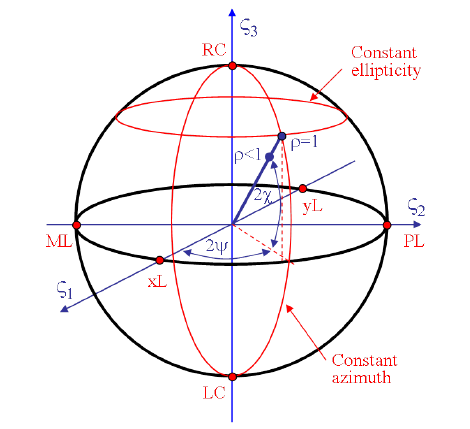
\includegraphics[width = 0.6\textwidth]{figures/Pincore_1.png}
% \caption{Rotation of the optical field components by rotator}
% \label{fig:poincar}
%\end{figure}
%
%Figure \ref{fig:poincar} shows the poincar\'e sphere. Prior to describe this figure, it is useful to recall the relations between elliptical parameters $\psi$, $\chi$ and $\alpha$ from Eq. \ref{Eq:nrStokesvec} and Eq. \ref{Eq:stokevector}:
%\begin{subequations}\label{Eq:PoincareEq1}
%	\begin{align}
%	 \cos 2\chi \cos 2\psi  =  \cos 2\alpha  = \frac{S_{1}}{S_{0}}  = \varsigma_{1}\\
%	 \cos 2\chi \cos 2\psi  =  \sin 2\alpha \cos \delta  = \frac{S_{2}}{S_{0}}  = \varsigma_{2} \\
%	 \sin 2\chi  =  \sin 2\alpha \sin \delta   = \frac{S_{3}}{S_{0}}  =\varsigma_{3}
%	\end{align}
%\end{subequations}
%
%The three parameters $\varsigma_{1}, \varsigma_{2}$ and $\varsigma_{3}$ are the three coordinates of the sphere as it is shown in Fig. \ref{fig:poincar}. The linearly polarized states are on the "equator", the $xL$ and $yL$ along $\varsigma_{1}$ axis represent the horizontal and vertical linearly polarized states respectively and the $PL$ and $ML$ along $\varsigma_{2}$ represent the $\pm 45^{\circ}$ respectively. The final axis $\varsigma_{3}$ represents the right ($RC$) and left ($LC$) circularly polarized states at the north and south poles of the sphere respectively. 
%In conclusion, all the "right-handed" elliptical states are on the Northern hemisphere, while the opposite holds for the "left-handed" states. As it is shown in Fig. \ref{fig:poincar}, the constant ellipticity is on the "parallels" and constant azimuth on the "meridians" and any partially polarized states can be represented by any points with in the sphere, while satisfying  $\varsigma_{1}+\varsigma_{2}+\varsigma_{3} = \rho^{2}$. The $\rho$ is the degree of polarization. This relation proves that totally un-polarized states are at the center of the sphere. 
%



%%%%%%%%%%%%%%%%%%%%%%%%%%%%%%%%%%%%%%%%%%%%%%%%%%%%%%%%%%%%%%%%%%%%%%%%%%%%%%
%%% CHAPTER 4
%%%%%%%%%%%%%%%%%%%%%%%%%%%%%%%%%%%%%%%%%%%%%%%%%%%%%%%%%%%%%%%%%%%%%%%%%%%%%
\chapter{Imaging Polarimetry}
\section{Introduction}
Imaging polarimetry refers to different approaches for describing propagation of polarized light and its interactions with optical system. Jones calculation and Stokes-Mueller representation both can be used for mathematical expression of the polarized system. However the Stokes-Mueller polarimetry is more suited for polarimetry applications due to two reasons. First the polarized light after interaction with the medium could be fully, partial or un-polarized and Jones calculus is only applicable for fully polarized light state. Second intensity measurements of polarized lights and experimental data are more desirable and Mueller formalism is based on experimental consideration of intensity measurements. Based on mentioned reasons, the Stokes-Mueller polarimetry is explained in the following. 

Stokes-Mueller polarimetry refers to measuring Stokes vector of Mueller matrix and it can be used either to highlight the different layers of the tissue by showing diffuse light coming from deeper layers and showing the medium response with different polarized conditions or it can be used to highlight some medium characteristics. Mueller matrix polarimetry should be used for the later application. 

 Stokes-Mueller polarimetry system contains two major elements; \textit{PSA}, polarization states analyser and \textit{PSG}, polarization states generator. The \textit{PSA} contains a set of elements which analyse the polarization state of incoming light and \textit{PSG} contains the elements which generate the polarization states. Three main subcategory of polarimetry are introduced by \cite{goldstein2003polarized}, which includes:
\begin{itemize}
	\item Rotating element polarimetry \\
	The Stokes vector and Mueller matrix parameters are measured here with rotating the polarized elements (polarizer, retarder). 	
	\item Oscillating element polarimetry \\
	Which rotates the polarization of light using some electro or magneto-optical device such as liquid crystal cell. 
	\item Phase modulation polarimetry \\
	These polarimeters use devices that vary in retardance in response to an electrical signal.
\end{itemize} 

However different types of imaging polarimetry systems had implemented in the literature which does not follow the mentioned category exactly. These systems are discussed with their details in section \ref{polState}.

\section{Optical Properties of Medium}

Beside the nature of the light and polarized states of incident light, we are interested to check the polarized properties of the optical elements and the subjected materials as well. A medium can have different optical properties such as, depolarization, birefringence (retardants) and diattenuation which are explained in the following. 
	\begin{itemize}
	\item \textbf{Depolarization}\\
	If an initial state of the light is 100$\%$ polarized and polarization degree of the existing state is less than unity, the system posses the depolarization property. Depolarization is usually encountered due to multiple scattering of photons although randomly oriented uniaxial birefringence can also create the depolarized state. The general form of a pure depolarization Mueller matrix is shown in Eq.\ref{Eq:DepolarizationMul}. Here $1-\vert a \vert$ and $1-\vert b \vert$ are depolarization factors for linear polarization states and $1-\vert c \vert$ represents depolarization factor for circular polarization. The net depolarization factor is shown in Eq. \ref{Eq:netDepolarizationfac}
	\begin{equation}\label{Eq:DepolarizationMul}
	\small
		M_{\Delta} = \begin{bmatrix}
	1 & & 0 & & 0 & & 0\\0 && a && 0 && 0\\ 0 && 0 && b && 0\\ 0 && 0 && 0 && c
	\end{bmatrix} , \hspace{1 cm} \vert a \vert, \vert b \vert, \vert c \vert \leq 1
	\end{equation}
	\begin{equation}\label{Eq:netDepolarizationfac}
	\small
		\Delta  = 1 - \frac{\vert a \vert + \vert b \vert + \vert c \vert }{3} = 1 - \frac{\vert tr (M_{\Delta}-1)\vert}{3} , \hspace{0.5 cm} 0\leq \Delta \leq 1
		\end{equation}		
	\item \textbf{Retardants}\\	
	Retardance is the phase shift between orthogonal components of polarized light and it occurs due to differences in refractive indices of different polarized states. 
	
	Birefringence is a linear retardants which occurs due to phase difference between orthogonal linear polarization states (between vertical and horizontal or between $45^{\circ}$ and $-45^{\circ}$ ). Mueller matrix of linear retardance ($\delta$) while its fast axis is rotated by angle $\theta$ with respect to the horizontal axis is shown in Eq.\ref{Eq:Birefringence}
	\begin{equation}\label{Eq:Birefringence}
	\small
	M_{R_{B}}=\begin{bmatrix}
	1 &&  0 &&  0  && 0\\
	0 && \cos^{2}2\theta +\sin^{2}2\theta\cos\delta && \sin 2\theta\cos 2\theta(1-\cos\delta) &&  -\sin 2\theta \sin \delta\\ 
	0 &&\sin 2\theta\cos 2\theta(1-\cos\delta) && \sin^{2}2\theta +\cos^{2}2\theta\cos\delta && \cos 2\theta \sin \delta\\
	 0 && \sin 2\theta \sin \delta && -\cos 2\theta \sin \delta && \cos\delta
	\end{bmatrix}
	\end{equation}	

	Beside linear retardance, there is circular retardance $\psi$ (optical rotation) as well, which arises due to phase difference between right circularly polarized (RCP) and left circularly polarized (LCP) states. The Mueller matrix for a circular retardance is shown in Eq.\ref{Eq:CircularRet}.
	\begin{equation}\label{Eq:CircularRet}
	\small
	M_{R_{C}}=\begin{bmatrix}
	1 &&  0 &&  0  && 0\\
	0 && \cos 2\psi && -\sin 2\psi &&  0\\ 
	0 && \sin 2\psi && \cos 2\psi && 0\\
	 0 && 0 && 0 && 1
	\end{bmatrix}
	\end{equation}
	
	\item \textbf{Diattenuation}\\
	Diattenuation $d$ of an optical elements corresponds to differential attenuation (absorption and scattering) of orthogonal polarizations for both linear and circular polarizations states. Accordingly linear diattenuation is defined as differential attenuation of two orthogonal linear polarization states and circular diattenuation is defined as differential attenuation of RCP and LCP. Mueller matrix of linear diattenuator is defined in Eq.\ref{Eq:LinearDiattenuation}. Two intensity transmittance (reflectance) parameters are used for orthogonal states ($q$, $r$). $\theta$ is the orientation angle of principal axis. 
	
	\begin{equation}\label{Eq:LinearDiattenuation}
	\small
	M_{D}=\begin{bmatrix}
	q+r &&  (q-r)\cos 2\theta &&  (q-r)\sin 2\theta && 0\\
	(q-r)\cos 2\theta && (q+r)\cos^{2}2\theta + 2\sqrt{(qr)}\sin^{2}2\theta && (q+r-2\sqrt{(qr)})\sin 2\theta\cos 2\theta & & 0\\ 
	(q-r)\sin 2\theta && (q+r-2\sqrt{(qr)})\sin 2\theta\cos 2\theta && (q+r)\cos^{2}2\theta + 2\sqrt{(qr)}\sin^{2}2\theta && 0\\
	 0 && 0 && 0 && 2\sqrt{(qr)}
	\end{bmatrix}
	\end{equation}		
	\end{itemize}


The mentioned optical properties of the tissue can be calculated using inverse polarimetry analysis based on Mueller matrix decomposition. The Lu-Chipman decomposition method \cite{lu1996interpretation} is a well known inverse polarimetry analysis which is explained in the following section.

\section{The Lu-Chipman Decomposition}
The proposed method of Lu-Chipman \cite{lu1996interpretation} allows a Mueller matrix to be decomposed into the product of three matrix of Diattenuation, Depolarization and Retardant (See Eq.\ref{Eq:LuchimpanDec}). In this representation $M_{\Delta}$ describes the depolarizing effects of the medium, $M_{R}$ shows the effects of linear birefringence and $M_{D}$ includes the effect of linear and circular diattenuation. 

 	\begin{equation}\label{Eq:LuchimpanDec}
	\small
	M\Leftarrow M_{\Delta}.M_{R}.M_{D}
	\end{equation}
Each of these matrices can be calculated and further be used to extract individual medium properties such as $d$ \textit{diattenuation} factor, $\Delta$ \textit{depolarization}, $\delta$ \textit{linear retardance}, rotation of retardance axis $\theta$ and a circular retardance $\psi$. Calculation of these parameters are explained step by step in the following. 

Lets start with the diattenuation matrix. This matrix can be described as:
	\begin{equation}\label{Eq:LCDiattenuator}\nonumber
	\small
	M_{D}=\begin{bmatrix}
	1 && \overrightarrow{d}^{T}\\ \overrightarrow{d} && m_{D}
	\end{bmatrix}
	\end{equation}
Where $m_{D}$ is a $3\times 3$ sub-matrix which is defined using the diattenuation vector $\overrightarrow{d}$. 
	\begin{subequations}\label{eq:Diatt}
	\small
	\begin{center}
	\begin{align}	
	\overrightarrow{d} = \frac{1}{M_{11}} \begin{bmatrix}
	M_{12} && M_{13} && M_{14}\end{bmatrix}^{T}\\
	d^{\wedge} = \frac{\overrightarrow{d}}{\vert \overrightarrow{d} \vert}\\
	\vert \overrightarrow{d} \vert =d = \frac{1}{M_{11}}\sqrt{M_{12}^{2}+M_{13}^{2}+M_{14}^{2}}\\
	m_{D} = \sqrt{(1-d^{2})}I+ (1-\sqrt{(1-d^{2})})d^{\wedge}d^{\wedge T}
	\end{align}
	\end{center}
	\end{subequations}

Using the diattenuation matrix, the other factors are computed (See Eq.\ref{eq:reformLCD}. 
	\begin{equation}\label{eq:reformLCD}
	\small
	M_{\Delta}M_{R} = M' = M M_{D}^{-1}
	\end{equation}
The depolarization matrix, $M_{\Delta}$ is written in the following form. Here $\overrightarrow{P}_{\Delta}$ is based on polarizance vector $\overrightarrow{P}$  and sub-matrix $m$ of the Mueller matrix $M$ (See Eq.\ref{eq:polarizance}) 
	\begin{equation}\label{eq:MDelta}
	%\small
	M_{\Delta} = \begin{bmatrix}
	1 && \overrightarrow{0}^{T}\\ \overrightarrow{P_{\Delta}} && m_{\Delta}
	\end{bmatrix}
	\end{equation}	
	\begin{subequations}\label{eq:polarizance}
	\small
	\begin{align}	
	\overrightarrow{P} = \frac{1}{M_{11}}\begin{bmatrix}
	M_{21} && M_{31} && M_{41}
	\end{bmatrix}^{T}\\
	\overrightarrow{P_{\Delta}} = \frac{(\overrightarrow{P} - m \overrightarrow{d})}{1-d^{2}}	
	\end{align}
	\end{subequations}
And $m_{\Delta}$ is the sub-matrix of $M_{\Delta}$ which is shown in Eq.\ref{eq:subMDelta}.
	\begin{equation}\label{eq:subMDelta}
	\small
	m_{\Delta} = \begin{bmatrix}
	a && 0 && 0\\
	0 && b && 0\\
	0 && 0 && c
	\end{bmatrix}	
	\end{equation}
The last factor is retardant matrix $M_{R}$. which can be reformed as follows (See Eq.\ref{eq:MR}). In this representation $m_{R}$ is the sub-matrix of $M_{R}$ and is computed using polarizance and diattenuation factors and sub-matrix of $M$ as it is presented in Eq.\ref{eq:subMR}
	\begin{equation}\label{eq:MR}
	\small
	M_{R} = \begin{bmatrix}
	1 && \overrightarrow{0}^{T}\\
	\overrightarrow{0} && m_{R}
	\end{bmatrix}	
	\end{equation}		
	
	\begin{equation}\label{eq:subMR}
	\small
	m_{R} = \frac{1}{\sqrt{(1-d^{2})}}[m - \frac{1-\sqrt{1-d^{2}}}{d^{2}}(\overrightarrow{P}.\overrightarrow{d}^{T})]
	\end{equation}
	
The combined effects of linear and circular retardance is computed by Eq.\ref{eq:TR}. 
	\begin{equation}\label{eq:TR}
	\small
	R = \cos^{-1}\lbrace{\frac{Tr(M_{R})}{2}-1 \rbrace}
	\end{equation}
Using the computed matrices and parameters, individual parameters of the medium can be computed, as it is listed in Table.\ref{Tab:ParMed}\\

	\begin{table}
	\small
	\begin{center}
	\caption{Medium Characteristics}
	\begin{tabular}{|c|c|c|}
	\hline
	Parameters & Notations & Equation \\
	\hline 
	& & \\
	 Linear retardance & $\delta$ & $ \cos^{-1}(\sqrt{[M_{R}(2,2)+ M_{R}(3,3)]^{2} +[M_{R}(3,2)+ M_{R}(2,3)]^{2}}-1)$\\
	 & & \\
	Optical rotation & $\psi$ & $\tan^{-1}[(M_{R}(3,2)-M_{R}(2,3))(M_{R}(2,2)-M_{R}(3,3))^{-1}]$\\
	& & \\
	Diattenuation & $d$ & $M_{D}(1,1)^{-1}\sqrt{M_{D}(1,2)^{2}+M_{D}(1,3)^{2}+M_{D}(1,4)^{2}}$\\
	& & \\
	Depolarization & $\Delta$ & $1 - \frac{\vert Tr (M_{\Delta}-1)\vert}{3}$\\
	& & \\
	\hline   
  	\end{tabular}
  	\label{Tab:ParMed}
  	\end{center}
	\end{table}

Since matrix multiplication is generally non commutative, one should concerns about the multiplication order of Lu-Chipman matrices and the effects displacement. The influence of these orders were investigated by \cite{ghosh2010influence}. Their results indicated that for the turbid media with weak diattenuation, the extracted polarization parameters are independent of the selected multiplication orders. These results were confirmed for biological tissues due to their weak diattenuation effects. Therefore it was concluded that individual tissue polarimetry effects can be successfully quantified despite their simultaneous occurrence, even in the presence of numerous complexities due to multiple scattering \cite{ghosh2010influence}.



%%\section{Polarized Light in Scattered Media} 
%%The propagation of the polarized light in a scattering medium is a complex process. Optical properties of the medium, such as shape, size, refractive index of the scattering particles as well as the polarization state of the incident light, all play important roles. Based on optical properties, the medium is divided into two categories, weakly (single) scattering and strongly (multiple) scattering. The optical thickness of the object for single scattering must be quite small in comparison with strong scattering media. The biological tissues are considered as turbid media and are categorized as strongly scattering media. 



\section{Polarimetry Systems in Biomedical field}
\label{polState}

Polarization has been used in biomedical field, specially for removing the multiple scattering component of the light beam. This task is done in order to enhance the contrast and achieve higher imaging resolutions. This technique has been used for years in skin imaging by dermatologists. Further the polarization effects are extensively used in various forms of biomedical light microscopy. Besides the mentioned polarization application, the full potential of polarization imaging in biomedicine has not been realized \cite{ghosh2011tissue}. Ghosh et al. \cite{ghosh2011tissue} summarizes the reasons as : 
	\begin{itemize}
	\item Extensive loss of polarization signal as a effect of tissue multiple scattering 
	\item Complicated nature of polarization effects in tissue
	\item Measurements difficulty, specially for small polarization signals
	\item Challenges in analysis and quantification of measured signals or images 
	\item Complexities in understanding and analysing the obtained results 
	\item Lack of detailed information on polarimetric properties of various tissues and their effects on polarized propagation.
	\end{itemize}
	
	Beside the mentioned challenges, several researchers are pursuing innovative solutions for this problem. Ghosh et al. \cite{ghosh2011tissue} provided a good summary on the current stage of the research in polarimtery and its problems.
	
	The polarimetry systems can be used either for tissue imaging or analysing optical characteristics of interested object. The tissue polarimetry can be applied either in terms of Stokes vector polarimeters or Mueller matrix polarimeters. The former technique is capable to define the polarization state of the backscattered light from the object, while the latter technique is able to detect the optical properties of the sample. 
	In following first the polarimetry systems as a non-conventional imaging system are discussed, then the Stokes vector polarimeters and finally the Mueller matrix polarimeter are reviewed. 
	
	\subsection{Polarimetry Imaging Systems}
	Beside the conventional use of cross polarized filters in dermoscope, the polarization and polarimetry systems have been used by several researchers as imaging techniques.
	
	
	Jacques et al \cite{Jacques12175282} was among the first researchers which considered to analyse the polarized images rather than single image for skin imaging. In his research he proposed the use of two polarised filters. polarizer generator was placed in the incident path in order to create the linearly polarized light illumination and polarizer analyser in the detection path. In this system the angle of the incident was chosen in a way that only backscattered light was collected with the camera. The authors proposed two image acquisition; one with the analysing polarizer oriented parallel to the illumination and one with the analyser positioned perpendicular to the illumination. The algebraic combination of these images ($I_{pol} = \frac{I_{par}-I_{per}}{I_{par}+I_{per}}$) leads to an image that emphasizes on the superficial skin structures which scattered the light rather than structures that absorb light \cite{Jacques12175282}. The authors used this imaging techniques for differentiation of clinical images of skin pathologies. 
	
The combination of co and cross polarized images $I_{pol}$ in addition to multispectral set up was used by \cite{yaroslavsky2003} as well. This set up was used for detection the boundaries of non melanoma parts with in the lesion. 

Another polarimetry system was proposed by \cite{boulbry2006novel}. They present a spectro-polarimetric system based on hemispherical backscattering for analysing skin lesions. Their system is capturing polarized light images without the effect of rough skin backscattering and It is composed of sixteen polarized light sources that provides, red, green or blue illumination and are distributed on a hemispherical shell in such a way that their incident beam collimated at the center of the hemisphere. 
A Stokes vector imaging is positioned on the shell at an oblique angle to the sample normal and consists of a 12 bits camera, two liquid crystal variable retarder and a fixed polarizer. Figure \ref{fig:SVhemisphere} shows the positioned of illumination source tubes over the hemisphere and the elements with in each tube (tri-color light emission diode, thin film polarizer and a lens)

	\begin{figure}
	\subfloat[]{%[width=0.3\textwidth]
	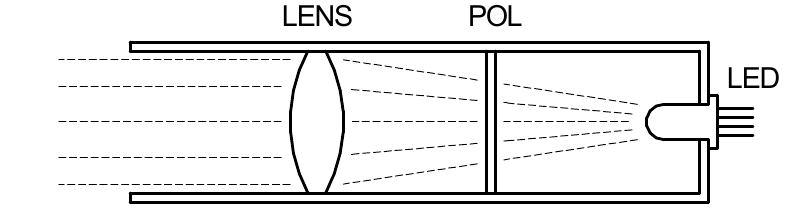
\includegraphics[width = 0.6\textwidth]{figures/fig1hemisphere.png}
	}\ \hfil
	\subfloat[]{%[width=0.3\textwidth]
    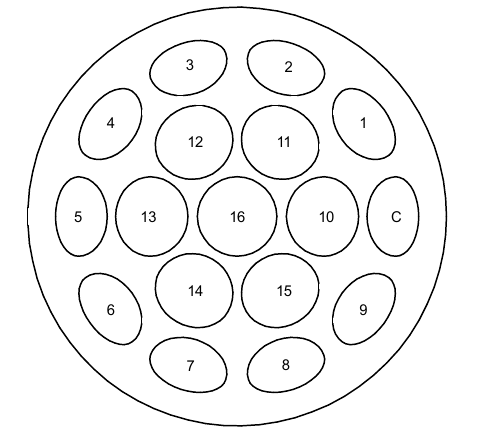
\includegraphics[height = 0.2\textheight , width = 0.35\textwidth]{figures/fig2hemispher.png}
	}
	\caption{(a)The illumination tubeand (b) Sixteen illumination tubes and the camera $C$, on the surface of the hemisphere with respect to the normal of the sample} 			 			    
	\label{fig:SVhemisphere}
	\end{figure}

The authors used their implemented system for measuring the Stokes parameters and respectively the un-polaized image. They also suggest to divide the polarized part of the measurements into two categories of reference polarized intensity and cross-polarized reference intensity.  


\cite{zhao2009} introduced an spectropolarimeter in order to acquire the spectral polarimetric and spatial characteristics changes of the tissue. Their spectropolarimeter consists of white light source which is directed to skin at an angle of $25^{\circ}$ with respect to the normal of the skin surface, a liquid crystal tunable filter (LCTF, 400-720 nm) and a CCD camera (see Fig.\ref{fig:spectropolarimeter}). The LCTF filter is manually aligned at four different angles ($0^{\circ}$, $45^{\circ}$, $90^{\circ}$, $135^{\circ}$) in front of the camera in order to achieve four images. The four image sequences are acquired at each waveband ($i_{0,\lambda}$, $i_{45,\lambda}$, $i_{90,\lambda}$, $i_{135,\lambda}$). The wavelengths are provided by LCTF within the visible range (400 - 720 nm).
The Stokes parameters are calculated based on raw measurements of the spectropolarimeter at different angles and reflectance measure of the white and black spectralon panels with spectrometer. \cite{zhao2009}.
		\begin{figure}
		\centering
		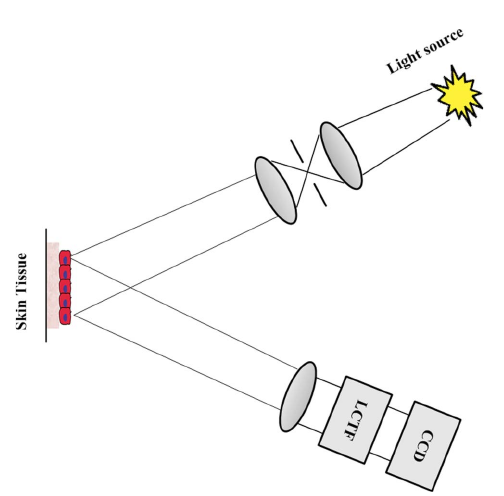
\includegraphics[width = 0.4\textwidth]{figures/spectropolarimeter.png}	
	\caption{The spectropolarimeter system developed by \cite{zhao2009}}
		\label{fig:spectropolarimeter}
		\end{figure}	 


The use of polarimeter in terms of Stokes measurements or imaging was proved that polarimetry imaging can be used to discriminate the pathological tissues and reveal biochemical and structural information of the tissue 



	
	\subsection{Stokes Vector Polarimeters}
	
	The measurement of four Stokes parameter was discussed in Sec. \ref{StokesMeasurement}. The explained set up was originally proposed by Collett et al. \cite{collett1984measurement}. This method was used by other researchers, such as \cite{ghosh2003depolarization,sankaran1999polarization,zhao2009,boulbry2006novel}, however when accurate quantification of the intrinsic tissue characteristics is required, a more sensitive approach should be considered. The sensitivity of the measurements can be improved by using a polarization modulation in combination with synchronous detection \cite{coa2004balanced,vitkin2002effects,studinski2000methodology,guo2006angular}. 
	
  	In \cite{coa2004balanced}, they demonstrate that it is possible to reduce the intensity noise and also direct measurements of Stokes parameters by using a amplitude or polarization modulation in combination with a phase-locked detector. 
  	
 \cite{vitkin2002effects} used polarization modulation with a synchronize detection in the perpendicular and backscattering orientations to detect the scattered light from the liquid turbid samples containing varying amounts of left and right isometric forms of a chiral sugar. Their research was aimed towards non-invasive techniques of glucose sensing in diabetic patients.   

A schematic of the experimental polarimetry system employing polarization modulation and synchronous detector with reference to \cite{guo2006angular,ghosh2011tissue} is shown in Fig.\ref{fig:PMSDpolarimetry}. In such a system, usually un-polarized light is passes through the mechanical chopper and then the lock-in amplifier in order to establish the overall signal intensity levels. A linear polarizer ($P_{1}$), with or without a quarter wave plate ($QWP_{1}$) is used as input optics. This set up is required in order to generate any of the four polarization states. The detection path consists of removable quarter wave plate ($QWP_{2}$) with its fast axis oriented at $-45^{\circ}$,  photoelastic modulator ($PEM$) and a linear polarizer, oriented at $45^{\circ}$. The linear polarizer converts the $PEM$ polarization modulation to intensity modulation suited for photo detection.

The PEM is a linearly birefringence resonant device, operating in $kHz$ range. The fast axis of the PEM is set to $0^{\circ}$ and its retardation is modulated according to the sinusoidal function $\delta_{PEM} = \delta_{0} \sin(\omega t)$. The $\delta_{0}$ is the user specified amplitude of the maximum retardation of $EPM$.

	\begin{figure}
	\centering 
	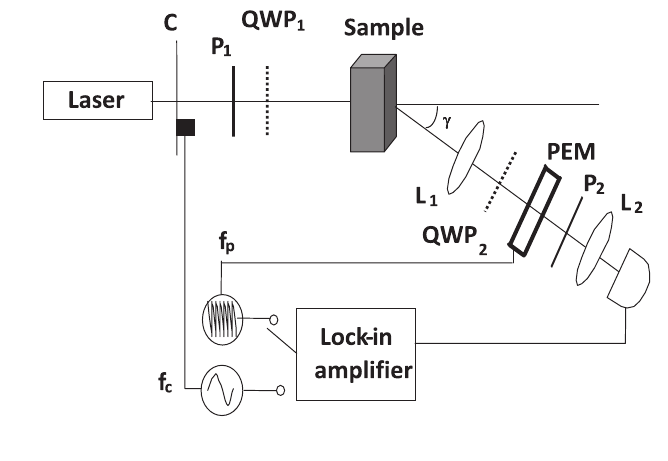
\includegraphics[width = 0.6\textwidth]{figures/PMSDpolarimetry.png}	
	\caption{ A schematic of the experimental polarimetry system with a polarization modulation and synchronous detector \cite{guo2006angular}}
	\label{fig:PMSDpolarimetry}
	\end{figure}

	
	\subsection{Mueller Matrix Polarimeter}
	As it was explained before, Stokes vectors are not enough for measuring the polarization transfer function of the sample and additional measurements and analysis is required. The sample polarization behaviour can be modelled by Mueller matrix. This matrix and its parameters was explained in Sec. \ref{MuellerMeasurement}. Sixteen elements of Mueller matrix can be measured via dc sequential static measurements or ac modulation based measurements \cite{ghosh2011tissue}. In both ways the four state of polarization (linear polarization at $0^{\circ}$, $45^{\circ}$, $90^{\circ}$ and rigth/left circular polaization $L$ and $R$) are applied individually as the input state, and the Stokes vector corresponding to each input are measured as an output. The 16 elements of the mueller matrix are then constructed using the measured Stokes vectors (see Eq. \ref{Eq:MuellerPolarimetry}) \cite{ghosh2008mueller}. 
	
	\begin{equation}\label{Eq:MuellerPolarimetry}
	\small
	M(i,j)= 
	\begin{bmatrix}
	\frac{1}{2}(I_{H}+I_{V}) &  \frac{1}{2}(I_{H}-I_{V}) &  I_{P}-M(1,1) &  I_{R}-M(1,1)\\
    \frac{1}{2}(Q_{H}+Q_{V}) &  \frac{1}{2}(Q_{H}-Q_{V}) &  Q_{P}-M(2,1) &  Q_{R}-M(2,1)\\
	\frac{1}{2}(U_{H}+U_{V}) &  \frac{1}{2}(U_{H}-U_{V}) &  U_{P}-M(3,1) &  U_{R}-M(3,1)\\
	\frac{1}{2}(V_{H}+V_{V}) &  \frac{1}{2}(V_{H}-V_{V}) &  V_{P}-M(4,1) &  V_{R}-M(4,1)\\		
	\end{bmatrix} 
	\end{equation}
	
Here the four input states are denoted with $H$ for $0^{\circ}$, $V$ for $ 90^{\circ}$, $P$ for $45^{\circ}$ and $R$ for right circular polarized. The Mueller matrix elements are represented by $M(i,j)$ with respect to their row and column.
	
The modulation/synchronous detection approach explained for Stokes polarimeter, can be used for Mueller polarimeter as well \cite{ghosh2008mueller,ghosh2009mueller}.

A dual rotating retarder approach is another way for generating the modulation-based Mueller matrix polarimeters \cite{ghosh2011tissue,goldstein1992mueller,azzam1978photopolarimetric,smith2002optimization}. In this approach the the incident polarization states are generated by the PSG unit which contains a linear polarizer and a rotating linear retarder (retardation $\sigma_{1}$, angular speed $\omega_{1}$) respectively. The backscattered light from the sample are then analysed by a PSA unit. This unit contains, a rotating linear retarder (retarder $\sigma_{2}$, synchronously rotating at angular speed $\omega_{2}$) and a fixed linear polarizer in sequence. In this set-up the axis of the polarizer and analyzer are kept parallel and the retardation of the two retarder are chosen to be the same $\sigma_{1} = \sigma_{2}= \pi/2$ while their angular frequencies differ from each other by five times ($\omega_{1} = \omega$, $\omega_{2} = 5\omega$ ). The rotation of the retarders at different rates result in a modulation of the detected signal and encodes all the sixteen Mueller matrix elements onto the amplitude and phases of 12 frequencies in the detected intensity signal. The detected signal is Fourier analyzed and the Mueller matrix elements are constructed from the Fourier coefficients \cite{ghosh2011tissue,goldstein1992mueller,azzam1978photopolarimetric,smith2002optimization}. \\

Dubreuil et al. \cite{dubreuil2007snapshot} introduced another modulation-based Mueller matrix polarimeter, known as Snapshot Mueller matrix. Snapshot system contains two linear birefringence retarder and a linear polarizer in PSG unit and two birefringence retarder and a fixed linear polarizer (perpendicular to the one in the PSG unit) at the PSA unit (see Fig. \ref{fig:snaphotMueller}). This technique measures the 16 elements of the Mueller matrix simultaneously by using wavelength polarization coding and decoding. The resulted spectral signal then is stored by the spectrometer and Fourier analysed in order to achieve the 16 elements of the Mueller matrix. 

	\begin{figure}
	\centering 
	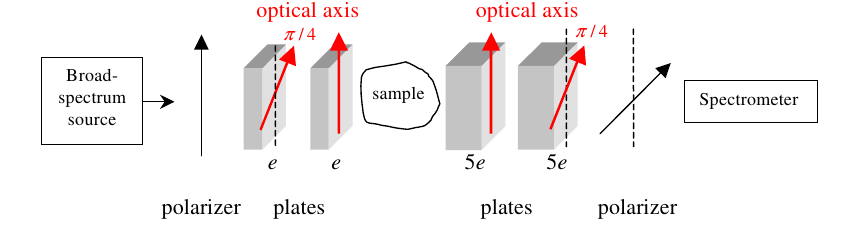
\includegraphics[width = 0.7\textwidth]{figures/snapshotMueller.png}	
	\caption{ Snapshot Mueller polarimeter for the configuration, \cite{dubreuil2007snapshot} }
	\label{fig:snaphotMueller}
	\end{figure}
	
Another polarimeter could be considered by using half wave plate $HWP$, linear polarizer and quarter wave plate $QWP$ as PSG unit respectively and a $QWP$ and another polarizer as PSA unit. In such a system (see Fig .\ref{fig:HWPQWPPQWPP}) different input polarized states are generated while the $HWP$ axis is kept at $45^{\circ}$ with reference to the incident polarizer (except for horizontally linear polarized state $H$ while HWP is parallel to polarizer). The QWP is removed for all polarized states except for right/left circular polarized states. For those situation, the $QWP$ is inserted in the PSG unit and its axis is rotated with reference to the linear polarizer by $\pm 45^{\circ}$. For such a system it is more convenient to measure the polarimetric matrix ($6\times4$) instead of Mueller matrix ($4\times4$). The row of this matrix are constructed with reference to the six input polarization states and the columns represent the Stokes vector output for each input state. This matrix is shown in Fig.\ref{fig:PolarimetricMatrix}. In this measurement, the first and second letter of each label indicate the input and output polarization state respectively and according to the polarimetric matrix, it could be seen that the output Stokes vector parameters are independent of the input polarization states. The advantage of this measurement relies on the fact that output Stokes parameters are normalized with relevant combination of orthogonal states. \\
 
	\begin{figure} [h]
	\centering 
	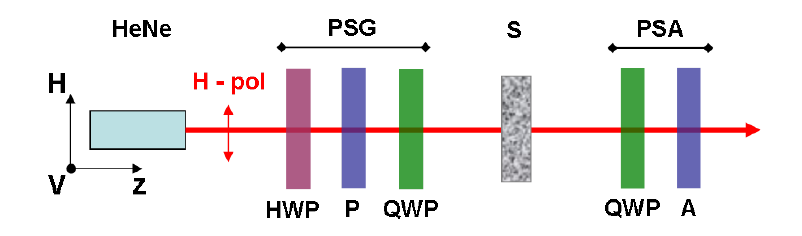
\includegraphics[width = 0.7\textwidth]{figures/HWPPQWP.png}	
	\caption{ Polarimetric matrix Polarimeter \cite{antonelli2011biomedical} }
	\label{fig:HWPQWPPQWPP}
	\end{figure}
	
	
	\begin{figure} [h]
	\centering 
	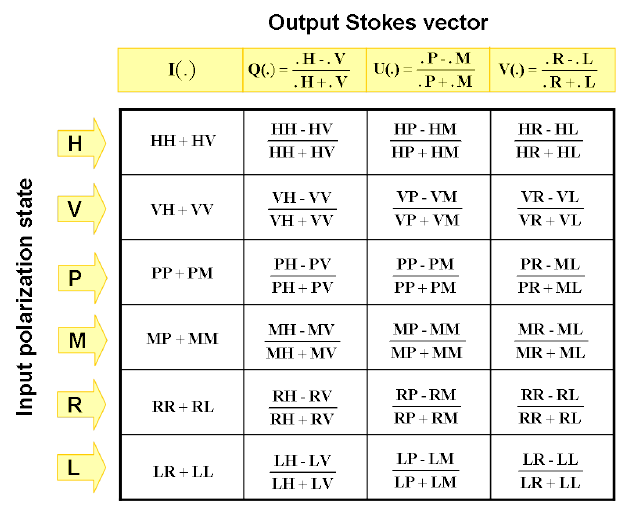
\includegraphics[width = 0.7\textwidth]{figures/PolarimetricMatrix.png}	
	\caption{ The polarimetric matrix\cite{antonelli2011biomedical} }
	\label{fig:PolarimetricMatrix}
	\end{figure}

The polarimeter systems mentioned so far are point polarimeter and are not feasible for large area imaging \cite{ghosh2011tissue}. The imaging polarimeter generally requires a dc, sequential measurements with different combination of polarized incident and detection states. Such a system will have lower sensitivity so alternative methods have been considered for instance using a liquid crystal variable retarders ($LC$) instead of manually rotating the optical parts of the PSG and PSA \cite{de2004general} (see Fig \ref{fig:LCMueller}).  The PSG unit of this system consists of a linear polarizer ($P_{1}$) and two liquid crystal variable retarders ($LC_{1}$, $LC_{2}$) with two retardance value of $\sigma_{1}$ and $\sigma{2}$ respectively. The PSA unit have a similar structure to PSG unit ($LC_{3}$, $LC_{4}$ and $P_{2}$) with the reverse order and the detection device at the end, in this case a CCD, for image acquisition. The structure of the LC polarimeter can be seen in Fig \ref{fig:LCMueller}.
	\begin{figure}
	\centering 
	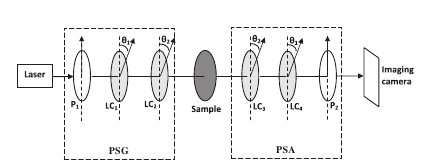
\includegraphics[width = 0.8\textwidth]{figures/LCMueller.png}	
	\caption{$LC$ Mueller matrix polarimeter \cite{ghosh2011tissue} }
	\label{fig:LCMueller}
	\end{figure}

Usually the birefringence axis of the two retarders are kept at angles $\theta_{1}$ and $\theta_{2}$ respectively with reference to the axis of the polarizer $P_{1}$. (Generally the angles are chosen as: $\theta_{1} = 45 ^{\circ}$ and $\theta_{2} = 0 ^{\circ}$). Considering the optics elements order in the PSG unit, once can conclude how the incident polarizer states can be related to $\sigma_{1}$ and $\sigma_{2}$. This relation is illustrated in Eq.\ref{Eq:LCMuellerEq}.

	\begin{equation}\label{Eq:LCMuellerEq}
	\small
	\begin{pmatrix} 
	I_{f}\\
	Q_{f}\\
	U_{f}\\	
	V_{f}\\
    \end{pmatrix} = 		
	\begin{pmatrix}
	1 & 0 & 0 & 0 \\
	0 & 1 & 0 & 0 \\
	0 & 0 & \cos \sigma_{2} &  \sin \sigma_{2}\\
	0 & 0 & -\sin \sigma_{2} &  \cos \sigma_{2}\\
	\end{pmatrix}
	\begin{pmatrix}
	1 & 0 & 0 & 0 \\
	0 & \cos \sigma_{1} & 0 & -\sin \sigma_{1} \\
	0 & 0 & 1 & 0 \\
	0 & \sin \sigma_{1} & 0 & \cos \sigma_{1} \\
	\end{pmatrix} 
	\begin{pmatrix}
	1\\
	1\\
	0\\
	0\\
	\end{pmatrix} = 
	\begin{pmatrix}
	1 \\
	\cos\sigma_{1}\\	
	\sin \sigma_{2} \sin \sigma_{1}\\
	\cos \sigma_{2} \sin \sigma_{1}\\
	\end{pmatrix}	
	\end{equation} 

According to Eq. \ref{Eq:LCMuellerEq}, only using the two angles of $\sigma_{1}$ and $\sigma_{2}$ the incident polarized states can be generated. In the same way the polarization states of the PSA unit can be applied \cite{de2004general}. For calculating the Mueller matrix in this system, the output of the PSG unit is considered in terms of a $4\times4$ matrix, called $W$. The columns of the $W$ are filled by the four incident polarized states . In the same way the output of the PSA unit is represented in terms of another $4\times4$ matrix called $A$. The rows of $A$ matrix represent the fours polarized states of the PSA unit. In this way 16 raw measurements are enough in order to create the measurement martix $B$ such as : 

	\begin{equation}
	\label{eq:LCMuellerEq}
	B = AMW
	\end{equation}
Here $M$ is the Mueller matrix of the sample which can be calculated by measuring the $B$ matrix and having the initial knowledge of $A$ and $W$. These two matrix can be known if the system is \textit{calibrated}\cite{compain1999general}.\\

%%%The calibration of a system like the imaging polarimeter we are describing is a very
%%%difficult task by the usual approach involving a detailed model of the instrument, as this
%%%system is a "stack" of many elements, each of which may introduce serious artefacts which
%%%may be difficult to understand and model properly.
%%%A very different approach has been followed at LPICM [70] to develop the eigenvalue
%%%calibration method (ECM), which has been successfully used on many different Mueller
%%%polarimeters. Without getting into details, which would be outside the scope of this
%%%manuscript, this method can accurately retrieve the matrices W and A from four mea-
%%%surements on calibration samples by linear algebra techniques, without any modelling of
%%%the instruments. Moreover, the calibration samples are not very specific (typically one
%%%can use linear polarizers, retardation plates other than half wave) and do not need to be
%%%accurately known, as they are characterized during the calibration procedure itself. Of
%%%course, our imaging polarimeter was calibrated at each wavelength by using ECM, and
%%%provided polarimetric images with a typical maximum error of the order of 0.02 to 0.03
%%%on the normalized elements Mij ∗
%%% = Mij /M11, i, j = 1..4 i · j = 1.

Recently Antonelli et al.\cite{antonelli2011biomedical} used several polarimeteric imaging techniques in order to analyse the optical properties of the medium, including; Full Mueller imaging system, Fourier space polarimetric imaging system  and Full Mueller real space imaging system. 

	\begin{figure}
	\begin{center}
	\subfloat[]{
	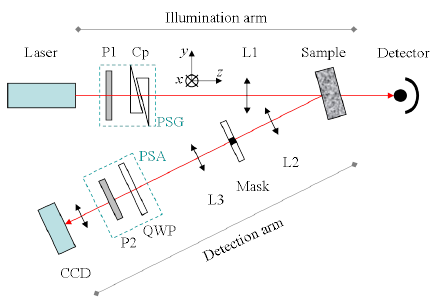
\includegraphics[width = 0.7\textwidth]{figures/illuminationMueller.png}
	\label{fig:focusedMueller}
	}\  \\
	\subfloat[]{%[width=0.3\textwidth]
    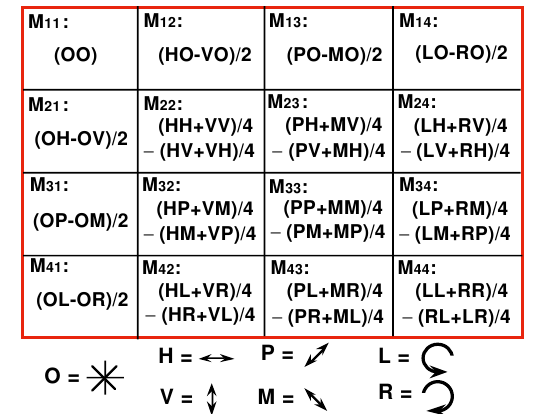
\includegraphics[width = 0.7\textwidth]{figures/illuminationMueller_table.png}
    \label{fig:illuminationMuellerTable}
	}
	\caption{(a)Full Mueller imaging system (b) Combination of the raw images for calculating the Mueller matrix elements   \cite{antonelli2011biomedical,hielscher1997diffuse}} 	
	\end{center}
	\end{figure}

The first instrument, Mueller polarimeter with focused illumination, was implemented according to the system described by \cite{hielscher1997diffuse}. Hielscher et al \cite{hielscher1997diffuse} developed the Mueller imaging system for analysing the intensity patterns of backscattered light from the turbid media. The developed system by \cite{antonelli2011biomedical} is shown in Fig.\ref{fig:focusedMueller}. In this system, a Helium-Neon (HeNe) laser source is used. The incident light is polarized after passing through the PSG unit. This unit consists of a dichroic plastic polarizer and a Babinet Soleil Bravais compensator ($Cp$). The polarizer is kept oriented horizontally in the x direction and the laser is rotated until total illumination intensity matched the dynamic range of the CCD. The compensator retarder is adjusted either on $180^{\circ}$ to obtain the linear polarized states ($H$, $V$, $P$, $M$) or $90^{\circ}$ in order to achieve the right and left circular polarized states ($R$, $L$). The lens $L_{1}$ is used to focus the polarized light onto the sample surface. A fraction of the polarized beam, transferred through the sample is measured by a detector as it is shown in Fig. \ref{fig:focusedMueller}, to obtain the photon mean free path. The backscattered light from the sample then is passing through $L_{2}$, $Mask$ and $L_{3}$ respectively prior to be analysed by the PSA unit. A $Mask$ is inserted in the focal plane of $L_{2}$ lens in order to remove the specular reflection of the laser beam on the front surface of the sample \cite{antonelli2011biomedical}. The PSA unit consists of a quarter wave plate and a plastic dichroic polarizer $P_{2}$. In case linear polarization state is desired the fast axis of $QWP$ and $P_{2}$ are kept parallel and for circular polarization state their axis is kept apart by $45^{\circ}$.\\

The 16 Mueller matrix elements using the mentioned system can be calculated by considering different polarized states of PSG and PSA units. In total considering 6 states for each unit 36 acquisition of raw images is required for completing the Mueller matrix. The polarization state of two unit for each element of the matrix is shown in Fig. \ref{fig:illuminationMuellerTable}. The first label indicates the polarization state of the PSG unit and the last label specifies the polarization state of the PSA unit. Label $O$ identifies the un-polarized state. \cite{antonelli2011biomedical,hielscher1997diffuse}. \\

The second polarimeter based on Fourier space is an extension of the method illustrated in Fig.\ref{fig:HWPQWPPQWPP}. This system is shown in Fig.\ref{fig:FourierTransformSystem}. The setup consists of PSG and PSA units, HeNe laser source, $FT$ lens, imaging lens $L_{1}$ and CCD ($M_{1}$ and $M_{2}$ are mirrors and used due to space limitations). The results of this system was evaluated using the polarimetric matrix instead of Mueller matrix. \\

	\begin{figure}
	\centering 
	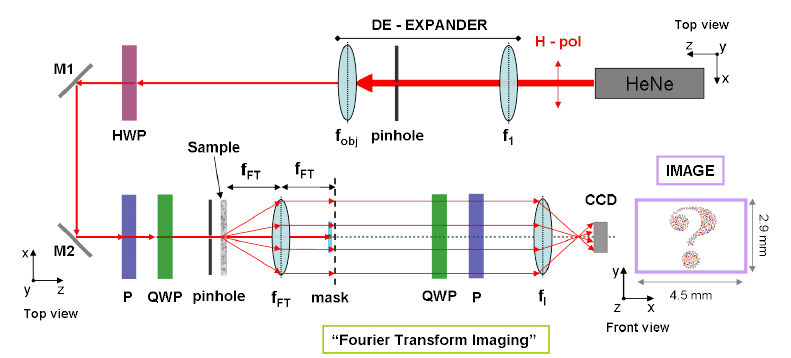
\includegraphics[width = 0.9\textwidth]{figures/FourierTransformImaging.png}	
	\caption{Structure of complete Fourier imaging polarimeter.\cite{antonelli2011biomedical}}
	\label{fig:FourierTransformSystem}
	\end{figure}


The last implemented system by \cite{antonelli2011biomedical} is called Real space Mueller imaging. This set up is very similar to the one developed by \cite{de2004general}, where both PSG and PSA units consists of a linear polarizer and two liquid crystal variable retarder (See Fig.\ref{fig:RealMueller}). In this system the halogen light source is used, the light source first passes through a diffuser and then a condenser, then through the PSG unit. The backscattered light from the sample are passing through PSA unit and then through interference filters with their wavelengths varying in the range of 500-700 nm. Before the zoom, a close-up lens is used to form a virtual image at a far enough distance from the lens to allow easy focussing. The zoom of the CCD camera provides the diversity option between $2\times2 cm^{2}$ or $6\times6 cm^{2}$ of field of view. 

	\begin{figure}[h]
	\centering 
	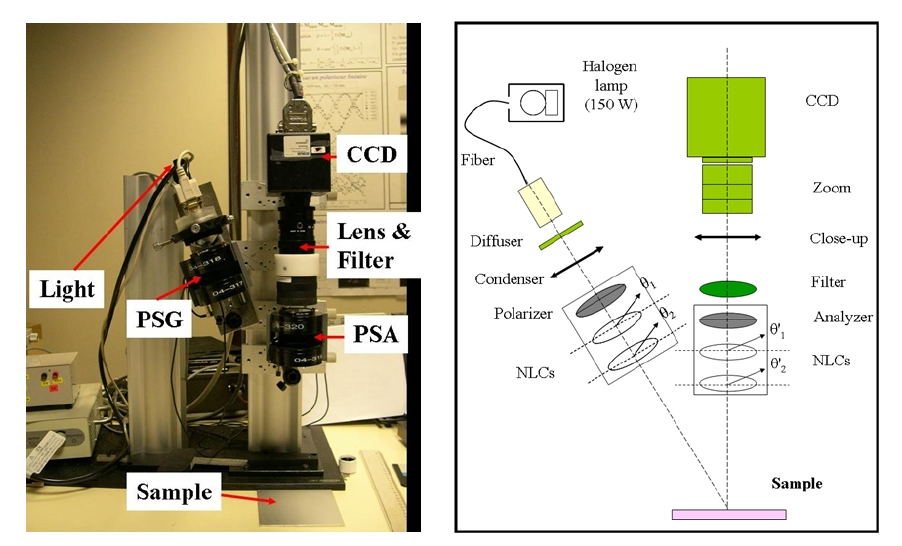
\includegraphics[width = 0.9\textwidth]{figures/RealMuellerImagingSystem.png}	
	\caption{Real space Mueller imaging.\cite{antonelli2011biomedical}}
	\label{fig:RealMueller}
	\end{figure}







%%%\cite{dubreuil2007snapshot}
%%%\cite{baba2002development}
%%%de2004general












%%In \cite{boulvert2005analysis}, author analyses the polarimetric properties of skin samples. Irritated pig skins were analysed and Mueller matrix were measured under different wavelengths.
%%A burn is a cutaneous lesion, caused either by contact with a heat source, chemicals, electricity or further to some exposure to radiations such as IR, UV, X-Rays or gamma rays. The skin cells will deteriorated as a result of burn. The damages of skin burns are divided into three degrees depending on the severity of the damages to the skin layers and underlying tissues. First degree burns affects only the epidermis while the third degree involves completer destruction of the fullest depth of the skin and underlying tissue.
%%
%%When light strikes the skin, small portion of light ($4-7\%$) is reflected by the outer layer of skin. The reminder of the light is propagated in the tissues. This portion is either absorbed or diffused by water, hemoglobin and melanine or transmitted through the skin.(see Figure \ref{fig:ProLigSki}).
%%	\begin{figure}
%%	\subfloat[]{%[width=0.3\textwidth]
%%	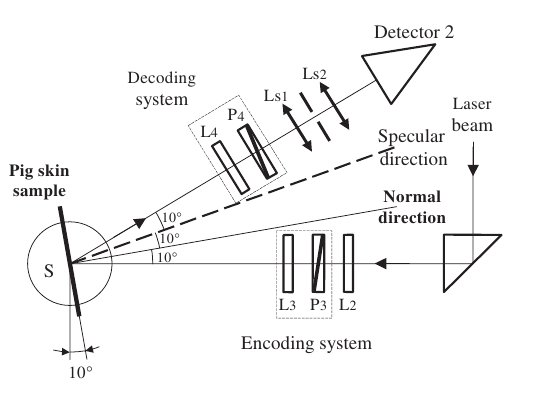
\includegraphics[width = 0.6\textwidth]{figures/ExpSetupPigSkin.png}
%%	}\ \hfil
%%	\subfloat[]{%[width=0.3\textwidth]
%%    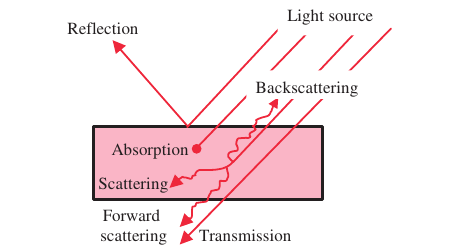
\includegraphics[height = 0.2\textheight , width = 0.35\textwidth]{figures/PropagationOfLight.png}
%%	}
%%	\caption{(a) Backscattering configurations experimental set up, (b) Propagation of light while striking the tissue}
%% 	\label{fig:ProLigSki}
%%	\end{figure}
%%
%%The research concludes that with measuring the polarization parameters, 70 days after the irradiation of living pig, it is possible to distinguish between a healthy skin sample and a 15 Gy or 20 Gy irradiated one. The research also conclude that depolarization will increase with decreasing of wavelengths (see figure.\ref{fig:DepWave})	
%%
%%In \cite{boulvert2007comparison}, the author analyses the polarization characteristics of the Mueller matrix via entropy factors and for weakly media such as pig skins after irradiation, they introduced another factor as polarization memory rate.
%%The Mueller coherence matrix $[C]$ is calculated from Mueller matrix using the Dirac matrices basis, while The $\lambda_{i}$ are the eigenvalues of hermitian matrix.  
%%	\begin{equation}ic
%%	\footnotesize
%%	[C]= 1/4 \sum_{i,j=0}^{3} M_{ij}\eta_{ij} = \lambda_{0}[C_{0}]+\lambda_{1}[C_{1}]+\lambda_{2}[C_{2}]+\lambda_{3}[C_{3}]
%%	\label{eq:MuellerCoherence}
%%	\end{equation}
%%
%%The Entropy of the Mueller matrix could be calculated from the eigenvalues of coherence-matrix 
%%	\begin{equation}
%%	\footnotesize
%%	E = - \sum_{i=0}^{3} P_{i}\log_{4}(P_{i}); \hspace{0.5 cm} P_{i}=\frac{\lambda_{i}}{\sum_{j=0}^{3}\lambda_{j}} \hspace{0.5 cm} 0\leq E \leq 1
%%	\end{equation}
%%
%%The entropy of isotropic and anisotropic depolarization can be separated by the following equations: 
%%	\begin{subequations}
%%	\footnotesize
%%	\begin{align}
%%	E_{iso} = -\frac{3P_{D}+1}{4}\log_{4}(\frac{3P_{D}+1}{4})-3\frac{1-P_{D}}{4}\log_{4}(\frac{1-P_{D}}{4})\\
%%	E_{ansio} = E_{iso}-\frac{1}{2m_{00}}\sum_{i=1}^{3}\lambda_{i}\log_{4}(\frac{2\lambda_{i}}{m_{00}(1-P_{D})})	
%%	\end{align}
%%	\label{eq:Eisoandaniso}
%%	\end{subequations}
%%Polarization memory $\Gamma$ is the ratio of the $P_{C}$ to $P_{L}$, which appears to work and better for the case of irradiation of skin with different dose of radiation.
%%\begin{figure}
%%	\centering
%%	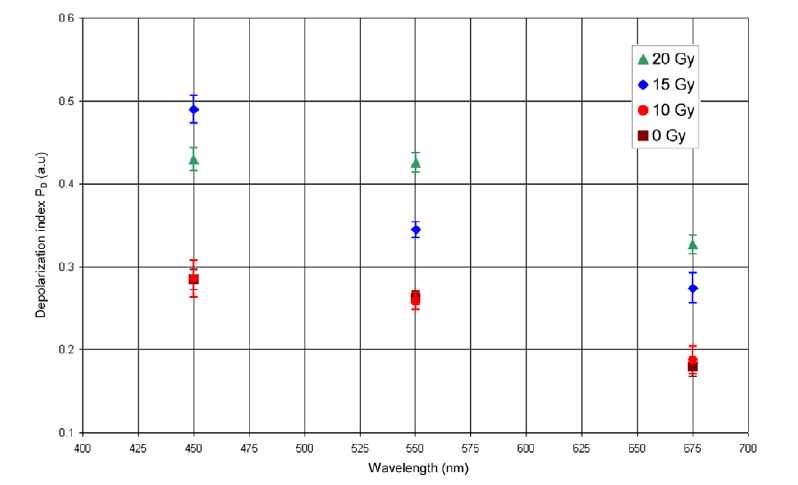
\includegraphics[width = 0.6\textwidth]{figures/DepolarizationvsWavelengthWGy.png}
%%	\caption{Depolarization index versus wavelength (nm)}
%%	\label{fig:DepWave}
%%	\end{figure}
%%\section{Boulbry et al, \cite{boulbry2006novel}}
%%\textit{A novel hemispherical spectro-polarimetric scattering instrument for skin lesion imaging, \cite{boulbry2006novel}}\\
%%In this papers the author introduces a spectro-polarimetric instrument based on hemispherical backscattering. 
%%The system is composed of sixteen polarized light sources that provides red, green or blue illumination. The light sources are distributed on a hemispherical shell, and each source produces a collimated beam incident on the center of the hemisphere. A Stokes vector imaging system is mounted on the shell at an oblique angle to the sample normal and consists of a 12-bit scientific camera, two liquid crystal variable retarders, and a fixed polarizer. Stokes vector images of light scattered towards the camera direction are generated for each source.
%%
%%\textbf{Using $I_{unpol}$, $I_{pol}$, and their imaging systems , Should be referred to the formulas}
%%







%%%%\chapter{Single Lesion Analysis}
%%%%
%%%%\section{Feature Selection}
%%%%Due to the nature of the problem and being able to visualize the pigmented lesions, the clinicians use some features of the lesion in order to differentiate the suspicious and benign lesions. The definition of these features depend on the diagnosis method. A lot of researches have been dedicated to computerize the process of finding and classifying these features. In order to achieve this goal, they tried to used the images of the lesions in order to retrieve either clinical or dermoscopic features.
%%%%
%%%%
%%%% diagnosis and differentiation of the pigmented lesion between the two class of suspicious and benign, depends on the feature


\bibliography{Literature}




\end{document}
